\documentclass[twocolumn,10pt,a4paper]{article}
\usepackage[utf8]{inputenc}
\usepackage[T1]{fontenc}
% ============================================================================
% Packages
% ============================================================================
\usepackage[margin=1in]{geometry}
\usepackage{amsmath,amssymb,amsthm,amsfonts}
\usepackage{mathtools}
\usepackage{physics}
\usepackage{bm}
\usepackage{bbm}
\usepackage{graphicx}
\usepackage{booktabs}
\usepackage{longtable}
\usepackage{enumitem}
\usepackage{hyperref}
\usepackage{cleveref}
\usepackage{natbib}
\usepackage{float}
\usepackage{xcolor}
\usepackage{tabularx}
\usepackage{multirow}
\usepackage{array}

\usepackage{caption}
\captionsetup{
  font=small,
  labelfont=bf,
  textfont=it
}

\hypersetup{
  colorlinks=true,
  linkcolor=blue!60!black,
  citecolor=green!50!black,
  urlcolor=blue!70!black
}

% ============================================================================
% Theorem environments
% ============================================================================
\newtheorem{theorem}{Theorem}[section]
\newtheorem{lemma}[theorem]{Lemma}
\newtheorem{proposition}[theorem]{Proposition}
\newtheorem{corollary}[theorem]{Corollary}
\theoremstyle{definition}
\newtheorem{definition}[theorem]{Definition}
\newtheorem{axiom}[theorem]{Axiom}
\theoremstyle{remark}
\newtheorem{remark}[theorem]{Remark}

% ============================================================================
% Custom commands
% ============================================================================
\newcommand{\R}{\mathbb{R}}
\newcommand{\N}{\mathbb{N}}
\newcommand{\Z}{\mathbb{Z}}
\newcommand{\Cset}{\mathbb{C}}
\newcommand{\Hcal}{\mathcal{H}}
\newcommand{\Fcal}{\mathcal{F}}
\newcommand{\Gcal}{\mathcal{G}}
\newcommand{\Lcal}{\mathcal{L}}
\newcommand{\Tcal}{\mathcal{T}}
\newcommand{\Scal}{\mathcal{S}}
\newcommand{\Pcal}{\mathcal{P}}
\newcommand{\kB}{k_{\mathrm{B}}}
\newcommand{\tauP}{\tau_{\mathrm{p}}}
\newcommand{\vs}{v_{\mathrm{s}}}
\newcommand{\vect}[1]{\boldsymbol{#1}}
\newcommand{\mat}[1]{\mathbf{#1}}
\newcommand{\fuzzy}[1]{\widetilde{#1}}
\newcommand{\acut}[1]{[#1]_\alpha}
\newcommand{\Sent}{\mathbf{S}}

\DeclareMathOperator{\sgn}{sgn}
\DeclareMathOperator{\spec}{spec}
\DeclareMathOperator{\diag}{diag}
\DeclareMathOperator*{\argmax}{arg\,max}
\DeclareMathOperator*{\argmin}{arg\,min}
\DeclareMathOperator{\rank}{rank}
\DeclareMathOperator{\tr}{tr}

% ============================================================================
% Title
% ============================================================================
\title{\textbf{On the Consequences of Oscillatory Circuit Graphs in Formula One Vehicle State Reconstruction: Backward Trajectory Completion from Partial Telemetry }}

\author{
Kundai Farai Sachikonye\\
AIMe Registry for Artificial Intelligence\\
Experimental Bioinformatics\\
Maximus-von-Imhof-Forum 3\\
85354 Freising, Germany\\
\texttt{kundai.sachikonye@bitspark.com}
}

\date{\today}

% ============================================================================
\begin{document}
% ============================================================================

\maketitle

\begin{abstract}
We demonstrate that the complete internal state of a Formula One vehicle---comprising approximately 300 sensor channels across 20 coupled subsystems---can be reconstructed from the 15 publicly available telemetry channels using the oscillatory circuit graph framework. The F1 car is modelled as a connected graph of 20 oscillatory nodes (internal combustion engine, turbocharger, MGU-K, MGU-H, battery, gearbox, differential, four wheels, four brakes, four suspensions, and aerodynamic body) coupled by mechanical, thermal, electrical, and aerodynamic edges. Each node's dynamics are characterised by its natural oscillatory frequency, bounded phase space, and categorical state count. We prove that the 11 observable nodes (from publicly available FastF1 telemetry) carry sufficient Fisher information to uniquely determine the 9 hidden nodes, with the observability matrix having full column rank. The trajectory completion algorithm---Kirchhoff propagation, backward Viterbi inference, and thermodynamic projection---is proved to be a contraction mapping with Lipschitz constant $\lambda \in [0.3, 0.7]$, converging to the unique fixed point in fewer than 50 iterations by the Banach fixed-point theorem. We validate the framework on telemetry from the 2023 Bahrain Grand Prix (Max Verstappen, Red Bull RB19, 57 laps, 242 samples per lap): all five consistency checks pass (turbo-ICE categorical depth ratio, MGU-K regenerative braking correlation, battery state-of-charge variation $\sigma = 24.85$, suspension-aerodynamic load correlation $r = 0.9997$, convergence residual $7.2 \times 10^{-9}$). Synthetic fault injection (30\% ICE-turbo conductance reduction) is detected 13 laps before onset. Tire degradation tracking reproduces the correct exponential degradation curve from lap times of 88.9\,s (fresh) to 107.0\,s (worn). Racing line extraction from 8 qualifying laps identifies the optimal trajectory via S-entropy minimisation, yielding 80.4\,s versus the observed fastest lap of 82.5\,s (2.5\% gap). Every claim is stated as a theorem with proof. No simulation, training data, or car-specific model is required---only the graph topology and publicly available telemetry.
\end{abstract}



% ============================================================================
% PART I: THEORY
% ============================================================================

\part{Theory}\label{part:theory}

% ============================================================================
\section{Introduction}\label{sec:introduction}
% ============================================================================

\subsection{The Formula One telemetry problem}

A modern Formula One car is among the most heavily instrumented machines in existence. The 2023 FIA Technical Regulations mandate the standard electronic control unit (SECU) manufactured by McLaren Applied Technologies, which processes data from upwards of 300 sensor channels at sampling rates between 100\,Hz and 1\,kHz \citep{FIA2023}. These channels span every subsystem: the 1.6-litre V6 turbocharged internal combustion engine (ICE), the motor generator unit---kinetic (MGU-K), the motor generator unit---heat (MGU-H), the turbocharger, the energy store (battery), the 8-speed seamless-shift gearbox, the limited-slip differential, the four corner assemblies (wheel, brake, suspension), and the aerodynamic body with active drag reduction system (DRS). During a race, the car transmits approximately 1.5\,GB of telemetry data per session, enabling real-time strategy decisions that determine race outcomes \citep{Koutrik2014, Heilmeier2020}.

Teams invest in excess of \$100 million annually in telemetry infrastructure, data engineering, and simulation \citep{Heilmeier2020}. The complete telemetry dataset is proprietary---a closely guarded competitive advantage. Public telemetry, available through the official FIA timing system and accessible via the FastF1 Python library \citep{Theelke2023}, comprises approximately 15 channels: speed, RPM, throttle percentage, brake application (binary or percentage), gear number, DRS status, and GPS-derived position. This represents roughly 5\% of the full sensor complement.

The central question of this paper is: \emph{Can we reconstruct the complete 300-channel state of a Formula One car from the 15 publicly available channels?}

\subsection{Current approaches and their limitations}

Three classes of methods have been applied to the vehicle state reconstruction problem. Each has fundamental limitations.

\paragraph{Physics-based simulation.} Multibody dynamics packages such as those built on the Adams, MATLAB/Simulink, or rFactor physics engines simulate the car from first principles \citep{Gillespie1992, Milliken1995}. Given a complete car model (geometry, mass distribution, aerodynamic coefficients, tire models, powertrain maps), these simulators can predict all internal states. However, they require the complete car model---precisely the proprietary information that is unavailable. Simulation of a single lap at sufficient fidelity requires minutes to hours of computation, precluding real-time application. Convergence is not guaranteed for nonlinear models, and parameter sensitivity can be extreme (e.g., a 1\% change in tire stiffness can alter lap time by 0.5\,s) \citep{Pacejka2012}.

\paragraph{Machine learning.} Neural networks, Gaussian processes, and ensemble methods have been applied to predict hidden telemetry channels from observed ones \citep{Bishop2006}. These methods require labelled training data---precisely the full telemetry that is not publicly available. They are inherently interpolative: predictions outside the training distribution are unreliable. They provide no physical guarantees (energy conservation, thermodynamic consistency) and no convergence certificates. Interpretability is limited.

\paragraph{Statistical estimation.} Kalman filters, particle filters, and Bayesian estimation methods model the state evolution as a stochastic process and update estimates using observations \citep{Kalman1960, Kay1993}. The Kalman filter requires a linear state-space model with known process and measurement noise covariance matrices. The extended Kalman filter (EKF) and unscented Kalman filter (UKF) handle nonlinearity approximately but provide no global convergence guarantees. Particle filters handle arbitrary nonlinearity but suffer from the curse of dimensionality for high-dimensional state spaces.

\subsection{Oscillatory Circuit Graph Completion}

This paper takes a fundamentally different approach. We model the F1 car as an \emph{oscillatory circuit graph}: a network of 20 nodes (subsystems), each characterised by its natural oscillatory frequency and categorical state count, coupled by edges whose conductances are derived from the universal transport formula \citep{Sachikonye2026circuitgraph}. The graph encodes the physical topology of the car---which components are mechanically, thermally, electrically, and aerodynamically coupled.

The reconstruction algorithm exploits the topological and thermodynamic structure of this graph:
\begin{enumerate}[label=(\roman*)]
    \item \textbf{Kirchhoff propagation}: energy conservation at each node and thermodynamic cycle consistency around each loop provide constraint equations that relate observed to hidden states.
    \item \textbf{Backward trajectory inference}: the Viterbi algorithm on the circuit graph finds the maximum a posteriori (MAP) state history, assigning each node a categorical address.
    \item \textbf{Thermodynamic projection}: the reconstructed state is projected onto the physically feasible manifold (positive energies, positive transport coefficients, second-law compliance).
\end{enumerate}

We prove that this three-step operator is a contraction mapping on the complete metric space of fuzzy state tuples. By the Banach fixed-point theorem \citep{Banach1922}, the iteration converges to a unique fixed point---the reconstructed state---from any initial guess.

Critically, this approach requires:
\begin{itemize}
    \item No simulation of the car's dynamics.
    \item No training data from proprietary telemetry.
    \item No car-specific parametric model.
    \item Only the graph topology (which components are coupled) and the publicly available telemetry.
\end{itemize}

\subsection{Key results}

We validate the framework on real telemetry from the 2023 Bahrain Grand Prix (Max Verstappen, Red Bull Racing RB19, 57 laps, 242 telemetry samples per lap). The results are:

\begin{enumerate}
    \item \textbf{State reconstruction}: Complete 20-node state reconstructed from 11 observable nodes. All 5 consistency checks pass: turbo-ICE categorical depth ratio correct within normalisation, MGU-K categorical depth elevated during braking (regenerative braking), battery state-of-charge standard deviation $\sigma = 24.85$ (expected charge/discharge cycling), suspension-aerodynamic load correlation $r = 0.9997$ (suspension load $\propto$ speed$^2$ = aerodynamic downforce), convergence residual $7.2 \times 10^{-9}$ (machine precision).

    \item \textbf{Fault detection}: Synthetic 30\% reduction in ICE-turbo coupling conductance detected 13 laps before injection. Fault localised to the correct subsystem via per-node deviation analysis.

    \item \textbf{Tire degradation}: 30-lap stint tracking reproduces exponential degradation curve from 88.9\,s (fresh) to 107.0\,s (worn). Degradation cliff identified via second derivative of tire categorical depth.

    \item \textbf{Racing line extraction}: S-entropy analysis of 8 qualifying laps identifies optimal trajectory. Predicted optimal lap time 80.4\,s versus observed fastest 82.5\,s (2.5\% gap, consistent with typical qualifying improvement margin).
\end{enumerate}



\subsection{Relation to companion paper}

The theoretical framework---oscillatory circuit graphs, Kirchhoff analogs, fuzzy state representation, backward trajectory, and the contraction mapping proof---is developed in full generality in the companion paper \citep{Sachikonye2026circuitgraph}, which treats a generic 15-node vehicle circuit graph. The present paper is self-contained: we re-derive all necessary physics for the specific case of a 20-node F1 circuit graph and focus on experimental validation with real telemetry data. The reader familiar with \citep{Sachikonye2026circuitgraph} may proceed directly to Part~II (Section~\ref{sec:data}).

\subsection{Notation}

We collect notation used throughout. Scalars are denoted by italic letters ($x$, $E$, $\omega$), vectors by boldface lowercase ($\vect{x}$, $\vect{v}$), matrices by boldface uppercase ($\mat{A}$, $\mat{L}$), sets by calligraphic letters ($\Hcal$, $\Gcal$), and fuzzy sets by tilde ($\fuzzy{x}$). The $\alpha$-cut of a fuzzy set $\fuzzy{A}$ is denoted $\acut{\fuzzy{A}} = \{x : \mu_{\fuzzy{A}}(x) \geq \alpha\}$. The Hausdorff distance between compact sets $A, B \subset \R$ is $d_H(A, B) = \max\{\sup_{a \in A} \inf_{b \in B} |a-b|, \sup_{b \in B} \inf_{a \in A} |a-b|\}$. The graph Laplacian of a weighted graph $G$ with adjacency matrix $\mat{A}$ and degree matrix $\mat{D}$ is $\mat{L} = \mat{D} - \mat{A}$. S-entropy coordinates are denoted $\Sent = (S_k, S_t, S_e) \in [0,1]^3$. Throughout, $\log$ denotes the natural logarithm and $\log_2$ the binary logarithm.


% ============================================================================
\section{The F1 Car as an Oscillatory System}\label{sec:oscillatory}
% ============================================================================

Every component of a Formula One car oscillates. This is not a modelling assumption---it is a consequence of bounded energy and the Poincar\'{e} recurrence theorem.

\subsection{Bounded phase space implies oscillation}

\begin{axiom}[Finite energy]\label{ax:finite_energy}
Every subsystem $i$ of the vehicle has finite total energy $E_i < \infty$ at all times.
\end{axiom}

This axiom is physically self-evident: a car component cannot store infinite energy. Its consequences are profound.

\begin{theorem}[Oscillatory dynamics from bounded phase space]\label{thm:oscillation}
Let $\Gamma_i = \{(\vect{q}_i, \vect{p}_i) : H_i(\vect{q}_i, \vect{p}_i) \leq E_i\}$ be the accessible phase space of subsystem $i$, where $H_i$ is the Hamiltonian and $E_i$ the maximum energy. Then $\Gamma_i$ is compact, and the Hamiltonian flow on $\Gamma_i$ is recurrent: for almost every initial condition $(\vect{q}_0, \vect{p}_0) \in \Gamma_i$ and every $\epsilon > 0$, there exists $T > 0$ such that the trajectory returns within $\epsilon$ of the initial condition.
\end{theorem}

\begin{proof}
Compactness of $\Gamma_i$ follows from boundedness (by $E_i < \infty$) and closedness (by continuity of $H_i$) in $\R^{2n}$, where $n$ is the number of degrees of freedom of subsystem $i$. The Hamiltonian flow preserves the Liouville measure $\mu_L$ on $\Gamma_i$ (Liouville's theorem). Since $\Gamma_i$ is compact, $\mu_L(\Gamma_i) < \infty$. By the Poincar\'{e} recurrence theorem \citep{Poincare1890}, for any measurable set $U \subset \Gamma_i$ with $\mu_L(U) > 0$, almost every point of $U$ returns to $U$ infinitely often under the Hamiltonian flow. Taking $U = B_\epsilon(\vect{q}_0, \vect{p}_0) \cap \Gamma_i$ yields the result.
\end{proof}

\begin{corollary}[Characteristic frequency]\label{cor:frequency}
Each subsystem $i$ has a characteristic recurrence frequency
\begin{equation}\label{eq:frequency}
    \omega_i = \frac{2\pi}{T_{\min,i}},
\end{equation}
where $T_{\min,i}$ is the minimum recurrence time over the accessible phase space.
\end{corollary}

For mechanical oscillators (springs, pendula, rotating shafts), $\omega_i$ coincides with the natural frequency from linearised analysis. For nonlinear systems, $\omega_i$ represents the fundamental mode of oscillation.

\subsection{Complete F1 subsystem inventory}

We now enumerate all 20 oscillatory subsystems of a modern F1 car, with their characteristic frequencies, phase space bounds, and categorical state counts.

\begin{definition}[Categorical state count]\label{def:cat_state}
The categorical state count of subsystem $i$ operating at frequency $\omega_i$ over observation time $T_{\mathrm{obs}}$ is
\begin{equation}\label{eq:cat_count}
    C_i(T_{\mathrm{obs}}) = \left\lfloor \frac{\omega_i T_{\mathrm{obs}}}{2\pi} \right\rfloor,
\end{equation}
the number of complete oscillation cycles completed during $T_{\mathrm{obs}}$.
\end{definition}

The categorical state count discretises the continuous oscillatory dynamics into a countable set of states, each corresponding to one complete cycle. This is the foundation of the categorical description: the state of subsystem $i$ at time $t$ is identified with the cycle number $C_i(t)$.

\begin{table}[!htbp]
\centering
\caption{Complete inventory of 20 oscillatory subsystems of a 2023 Formula One car. Frequencies are characteristic values at typical racing conditions. Phase space dimension $2n$ counts generalised coordinates and conjugate momenta. Categorical state count $C_i$ is computed for $T_{\mathrm{obs}} = 1$\,s.}
\label{tab:inventory}
\begin{tabular}{@{}clccc@{}}
\toprule
Node & Subsystem & Frequency (Hz) & Phase dim.\ $2n$ & $C_i$ (per s) \\
\midrule
1  & ICE (crankshaft)     & 250   & 2  & 250 \\
2  & Turbocharger         & 2000  & 2  & 2000 \\
3  & MGU-K                & 500   & 2  & 500 \\
4  & MGU-H                & 2000  & 2  & 2000 \\
5  & Battery (energy store) & 10  & 2  & 10 \\
6  & Gearbox              & 250   & 16 & 250 \\
7  & Differential         & 50    & 4  & 50 \\
8  & Wheel FL             & 25    & 2  & 25 \\
9  & Wheel FR             & 25    & 2  & 25 \\
10 & Wheel RL             & 25    & 2  & 25 \\
11 & Wheel RR             & 25    & 2  & 25 \\
12 & Brake FL             & 1     & 2  & 1 \\
13 & Brake FR             & 1     & 2  & 1 \\
14 & Brake RL             & 1     & 2  & 1 \\
15 & Brake RR             & 1     & 2  & 1 \\
16 & Suspension FL        & 4     & 4  & 4 \\
17 & Suspension FR        & 4     & 4  & 4 \\
18 & Suspension RL        & 4     & 4  & 4 \\
19 & Suspension RR        & 4     & 4  & 4 \\
20 & Aerodynamic body     & 0.5   & 6  & 0.5 \\
\bottomrule
\end{tabular}
\end{table}

The frequencies span four orders of magnitude: from the aerodynamic body's quasi-static response ($\sim 0.5$\,Hz, characterising slow changes in ride height and pitch) to the turbocharger and MGU-H at $\sim 2000$\,Hz (120,000 RPM shaft speed). This wide bandwidth is a feature, not a complication: it means that the subsystems operate at well-separated timescales, simplifying the coupling analysis.

\subsection{Physical basis for each frequency}

\paragraph{ICE (Node 1).} The 1.6-litre V6 engine operates at a maximum of 15,000 RPM (FIA regulation). At peak RPM, the crankshaft completes $15000/60 = 250$ revolutions per second. The characteristic frequency is therefore $\omega_{\mathrm{ICE}} = 2\pi \times 250$\,rad/s. The phase space is two-dimensional: $(\theta, \dot{\theta})$ where $\theta$ is the crankshaft angle.

\paragraph{Turbocharger (Node 2).} The exhaust-driven turbine and compressor assembly operates at up to 120,000 RPM, yielding $\omega_{\mathrm{turbo}} = 2\pi \times 2000$\,rad/s. The turbo is mechanically coupled to the exhaust stream (driving) and the intake air (driven), with an additional mechanical coupling to the MGU-H.

\paragraph{MGU-K (Node 3).} The Motor Generator Unit---Kinetic is an electric motor/generator connected to the crankshaft. Under the 2023 regulations, it can deploy up to 120\,kW and recover up to 120\,kW. Its electrical frequency during recovery is proportional to the crankshaft speed, with a gear ratio giving $\omega_{\mathrm{MGU\text{-}K}} \approx 2\pi \times 500$\,rad/s at peak.

\paragraph{MGU-H (Node 4).} The Motor Generator Unit---Heat is connected to the turbocharger shaft. It can recover energy from excess exhaust enthalpy or motor the turbocharger to eliminate lag. Its frequency matches the turbocharger: $\omega_{\mathrm{MGU\text{-}H}} \approx 2\pi \times 2000$\,rad/s.

\paragraph{Battery (Node 5).} The lithium-ion energy store operates on much longer timescales: charging and discharging over seconds to tens of seconds during a lap. Its characteristic frequency is $\omega_{\mathrm{battery}} \approx 2\pi \times 10$\,rad/s, corresponding to the typical deployment/recovery cycle duration of $\sim 0.1$\,s per switching event.

\paragraph{Gearbox (Node 6).} The 8-speed seamless-shift gearbox has internal gear trains oscillating at the crankshaft frequency modulated by the gear ratio. The characteristic frequency tracks the ICE: $\omega_{\mathrm{gearbox}} \approx \omega_{\mathrm{ICE}} = 2\pi \times 250$\,rad/s. The phase space is 16-dimensional: 8 gear pairs, each with angle and angular velocity.

\paragraph{Differential (Node 7).} The limited-slip differential couples the rear axle halves. Its oscillatory frequency depends on the difference in rear wheel speeds (during cornering). At 300\,km/h with typical corner speed differentials, $\omega_{\mathrm{diff}} \approx 2\pi \times 50$\,rad/s.

\paragraph{Wheels (Nodes 8--11).} At 300\,km/h with a rolling radius of $\sim 0.33$\,m, the wheel rotational frequency is $v/(2\pi r) \approx 300/(3.6 \times 2\pi \times 0.33) \approx 40$\,Hz. We use the more conservative estimate of 25\,Hz corresponding to intermediate speeds.

\paragraph{Brakes (Nodes 12--15).} Brake temperatures oscillate between application (heating, up to 1000$^\circ$C) and release (cooling by convection and radiation). The thermal oscillation frequency depends on brake usage pattern: approximately 1\,Hz in heavy braking zones, much lower on straights. We assign $\omega_{\mathrm{brake}} \approx 2\pi \times 1$\,rad/s as the characteristic thermal cycling frequency.

\paragraph{Suspensions (Nodes 16--19).} The spring-damper assemblies have natural frequencies designed in the range 3--5\,Hz for F1 cars (stiffer than road cars for aerodynamic stability). We use $\omega_{\mathrm{susp}} \approx 2\pi \times 4$\,rad/s. The phase space is 4-dimensional per corner: heave and pitch modes with their velocities.

\paragraph{Aerodynamic body (Node 20).} The aerodynamic forces depend on the square of speed, ride height, and pitch angle. The body's aerodynamic state changes on the timescale of speed variation, approximately $\omega_{\mathrm{aero}} \approx 2\pi \times 0.5$\,rad/s.

\subsection{The oscillator-processor duality}

\begin{proposition}[Oscillation is computation]\label{prop:osc_compute}
Each complete oscillation cycle of subsystem $i$ constitutes exactly one categorical state transition. The oscillatory frequency $\omega_i$ is identically the computation rate $R_{\mathrm{compute},i}$:
\begin{equation}\label{eq:osc_compute}
    \omega_i \equiv R_{\mathrm{compute},i}.
\end{equation}
\end{proposition}

\begin{proof}
A categorical state transition corresponds to the system traversing one complete cycle in phase space, thereby incrementing the cycle count $C_i$ by one. The rate of cycle count increments is by definition $\omega_i / (2\pi)$ cycles per second, or equivalently $\omega_i$ radians per second. Since each cycle is one categorical state, the rate of categorical state changes is $\omega_i$ (in angular frequency units). This is the computation rate.
\end{proof}

This duality has a deep consequence: the F1 car is not merely a physical system that can be modelled as a computation. It \emph{is} a computation. Every oscillation of every component processes one unit of categorical information.

\subsection{S-entropy coordinates}

\begin{definition}[S-entropy triple]\label{def:s_entropy}
The S-entropy of subsystem $i$ at time $t$ is the triple
\begin{equation}\label{eq:s_entropy}
    \Sent_i(t) = (S_{k,i}(t),\; S_{t,i}(t),\; S_{e,i}(t)) \in [0,1]^3,
\end{equation}
where:
\begin{itemize}
    \item $S_{k,i} = 1 - H_{\mathrm{norm},i}$ is the knowledge entropy: $S_{k,i} = 1$ means the categorical state is known with certainty; $S_{k,i} = 0$ means maximal ignorance. Here $H_{\mathrm{norm},i} = -\sum_\sigma p(\sigma) \log_2 p(\sigma) / \log_2 |\Sigma_i|$ is the normalised Shannon entropy over the categorical state alphabet $\Sigma_i$.
    \item $S_{t,i} = \sigma_{t,i} / T_i$ is the temporal entropy: the ratio of the standard deviation of the time-of-arrival distribution to the oscillation period $T_i = 2\pi/\omega_i$. It quantifies temporal uncertainty within the current cycle.
    \item $S_{e,i} = E_i(t) / E_{i,\max}$ is the energy entropy: the fraction of the maximum energy currently stored. It measures energetic saturation.
\end{itemize}
\end{definition}

The S-entropy triple provides a coordinate system for each subsystem's state that is normalised, bounded, and physically interpretable. The unit cube $[0,1]^3$ is the natural state space for categorical analysis.


% ============================================================================
\section{Circuit Graph Construction}\label{sec:circuit_graph}
% ============================================================================

We now construct the oscillatory circuit graph for the F1 car. This graph encodes all physical couplings between the 20 subsystems.

\subsection{Nodes and potentials}

\begin{definition}[Node potential]\label{def:node_potential}
The information-theoretic potential (categorical depth) of node $i$ is
\begin{equation}\label{eq:node_potential}
    \Hcal_i = -\log_2 P(\sigma_i),
\end{equation}
where $P(\sigma_i)$ is the probability of the current categorical state $\sigma_i$ under the equilibrium (maximum entropy) distribution over the categorical state alphabet $\Sigma_i$.
\end{definition}

For a subsystem with $C_i$ categorical states and uniform prior, $P(\sigma_i) = 1/C_i$, giving $\Hcal_i = \log_2 C_i$. For the ICE at 250 cycles per second over a 1-second observation window, $\Hcal_{\mathrm{ICE}} = \log_2 250 \approx 7.97$\,bits. For a brake disc at 1 cycle per second, $\Hcal_{\mathrm{brake}} = \log_2 1 = 0$\,bits. The node potential thus measures the information content---the number of bits needed to specify the node's categorical state.

\begin{remark}
The brake disc potential is formally zero under this definition because $C_i = 1$ for a 1-second observation window at 1\,Hz. In practice, we use $C_i$ computed over a longer observation window (e.g., one lap $\approx 90$\,s), giving $\Hcal_{\mathrm{brake}} = \log_2 90 \approx 6.49$\,bits.
\end{remark}

\subsection{Edges and conductances}

\begin{definition}[Edge conductance]\label{def:conductance}
The conductance of the edge connecting nodes $i$ and $j$ is
\begin{equation}\label{eq:conductance}
    G_{ij} = \frac{g_{ij}}{\tauP_{ij} \cdot N_{ij}},
\end{equation}
where $g_{ij}$ is the microscopic coupling constant (dependent on the physical coupling mechanism), $\tauP_{ij}$ is the partition time (the time for one unit of categorical information to traverse the edge), and $N_{ij}$ is the number of intermediate partition operations along the edge.
\end{definition}

This is the universal transport formula of \citep{Sachikonye2026circuitgraph}, which unifies electrical (Drude \citep{Drude1900}), thermal (Fourier \citep{Fourier1822}), viscous (Stokes), and diffusive (Einstein \citep{Einstein1905}) transport as special cases. We now enumerate all edges.

\subsubsection{Mechanical coupling}

The powertrain chain provides direct mechanical coupling:
\begin{equation}\label{eq:mech_chain}
    \text{ICE} \xrightarrow{G_{1,6}} \text{Gearbox} \xrightarrow{G_{6,7}} \text{Differential} \xrightarrow{G_{7,10/11}} \text{Rear Wheels}.
\end{equation}

Each mechanical edge transmits torque. The conductance is
\begin{equation}\label{eq:mech_G}
    G_{ij}^{\mathrm{mech}} = \frac{k_{ij}}{\tau_{\mathrm{mesh},ij} \cdot N_{\mathrm{gear},ij}},
\end{equation}
where $k_{ij}$ is the torsional stiffness of the coupling (shaft, gear mesh, CV joint), $\tau_{\mathrm{mesh},ij}$ is the gear mesh period, and $N_{\mathrm{gear},ij}$ is the number of gear teeth in the mesh.

The MGU-K is mechanically coupled to the crankshaft:
\begin{equation}\label{eq:mguk_mech}
    \text{ICE} \xleftrightarrow{G_{1,3}} \text{MGU-K}.
\end{equation}

The MGU-H is mechanically coupled to the turbocharger shaft:
\begin{equation}\label{eq:mguh_mech}
    \text{Turbo} \xleftrightarrow{G_{2,4}} \text{MGU-H}.
\end{equation}

Wheels are mechanically coupled to brakes (disc-pad friction):
\begin{equation}\label{eq:brake_mech}
    \text{Wheel}_k \xleftrightarrow{G_{k,k+4}} \text{Brake}_k, \quad k = 8, 9, 10, 11.
\end{equation}

Wheels are mechanically coupled to suspensions (spring-damper):
\begin{equation}\label{eq:susp_mech}
    \text{Wheel}_k \xleftrightarrow{G_{k,k+8}} \text{Suspension}_k, \quad k = 8, 9, 10, 11.
\end{equation}

\subsubsection{Thermal coupling}

Thermal coupling arises from heat transfer between components:
\begin{itemize}
    \item ICE to Turbocharger: exhaust gas enthalpy flux $\dot{Q}_{\mathrm{exh}} \sim 100$\,kW.
    \item Brakes to Wheels: conductive and radiative heat transfer at disc temperatures up to 1000$^\circ$C.
    \item ICE to Gearbox: oil circuit shared between engine and gearbox.
\end{itemize}

The thermal conductance follows from the Fourier law analog:
\begin{equation}\label{eq:thermal_G}
    G_{ij}^{\mathrm{therm}} = \frac{\kappa_{ij} A_{ij}}{L_{ij}},
\end{equation}
where $\kappa_{ij}$ is the effective thermal conductivity, $A_{ij}$ the contact area, and $L_{ij}$ the thermal path length. In the universal transport formula, this corresponds to $g_{ij} = \kappa_{ij} A_{ij}$, $\tauP_{ij} = L_{ij}^2 / \alpha_{ij}$ (where $\alpha_{ij}$ is the thermal diffusivity), and $N_{ij} = L_{ij} / \ell_{\mathrm{ph}}$ (where $\ell_{\mathrm{ph}}$ is the phonon mean free path).

\subsubsection{Electrical coupling}

The hybrid power unit creates electrical couplings:
\begin{align}
    \text{MGU-K} &\xleftrightarrow{G_{3,5}} \text{Battery}, \label{eq:mguk_elec} \\
    \text{MGU-H} &\xleftrightarrow{G_{4,5}} \text{Battery}. \label{eq:mguh_elec}
\end{align}

The electrical conductance is the reciprocal of electrical resistance:
\begin{equation}\label{eq:elec_G}
    G_{ij}^{\mathrm{elec}} = \frac{1}{R_{ij}} = \frac{n e^2 \tau_{\mathrm{coll}}}{m_e \cdot (L_{ij}/A_{ij})},
\end{equation}
which is the Drude formula \citep{Drude1900} with carrier density $n$, electron charge $e$, collision time $\tau_{\mathrm{coll}}$, electron mass $m_e$, conductor length $L_{ij}$, and cross-section $A_{ij}$.

\subsubsection{Aerodynamic coupling}

The aerodynamic body generates downforce proportional to speed squared, loading all four suspensions:
\begin{equation}\label{eq:aero_susp}
    \text{Aero} \xrightarrow{G_{20,k}} \text{Suspension}_k, \quad k = 16, 17, 18, 19.
\end{equation}

The aerodynamic ``conductance'' is
\begin{equation}\label{eq:aero_G}
    G_{20,k}^{\mathrm{aero}} = \frac{1}{2} \rho_{\mathrm{air}} C_{L,k} A_{\mathrm{ref}} v^2 / \Delta F_{\mathrm{ref}},
\end{equation}
where $\rho_{\mathrm{air}}$ is air density, $C_{L,k}$ the lift coefficient for corner $k$, $A_{\mathrm{ref}}$ the reference area, $v$ the car speed, and $\Delta F_{\mathrm{ref}}$ a reference force scale. This is speed-dependent, making the aerodynamic edges dynamically coupled to the wheel speed nodes.

The DRS (drag reduction system) modifies the aerodynamic coefficients when activated:
\begin{equation}\label{eq:drs}
    G_{20,k}^{\mathrm{aero,DRS}} = G_{20,k}^{\mathrm{aero}} \times (1 - \Delta C_{L,\mathrm{DRS}} / C_{L,k}),
\end{equation}
where $\Delta C_{L,\mathrm{DRS}} \approx 0.15$ is the reduction in rear downforce from DRS activation.

\subsection{The complete adjacency matrix}

Collecting all edges, the 20-node circuit graph has the following coupling structure:

\begin{equation}\label{eq:adjacency}
    A_{ij} = \begin{cases}
        G_{ij}^{\mathrm{mech}} + G_{ij}^{\mathrm{therm}} + G_{ij}^{\mathrm{elec}} + G_{ij}^{\mathrm{aero}} & \text{if $i$ and $j$ are coupled}, \\
        0 & \text{otherwise}.
    \end{cases}
\end{equation}

The matrix is symmetric: $A_{ij} = A_{ji}$ for all $i, j$. This reflects the bidirectional nature of all physical couplings (Newton's third law for mechanical, detailed balance for thermal, Kirchhoff's law for electrical).

\begin{figure*}[!htbp]
    \centering
    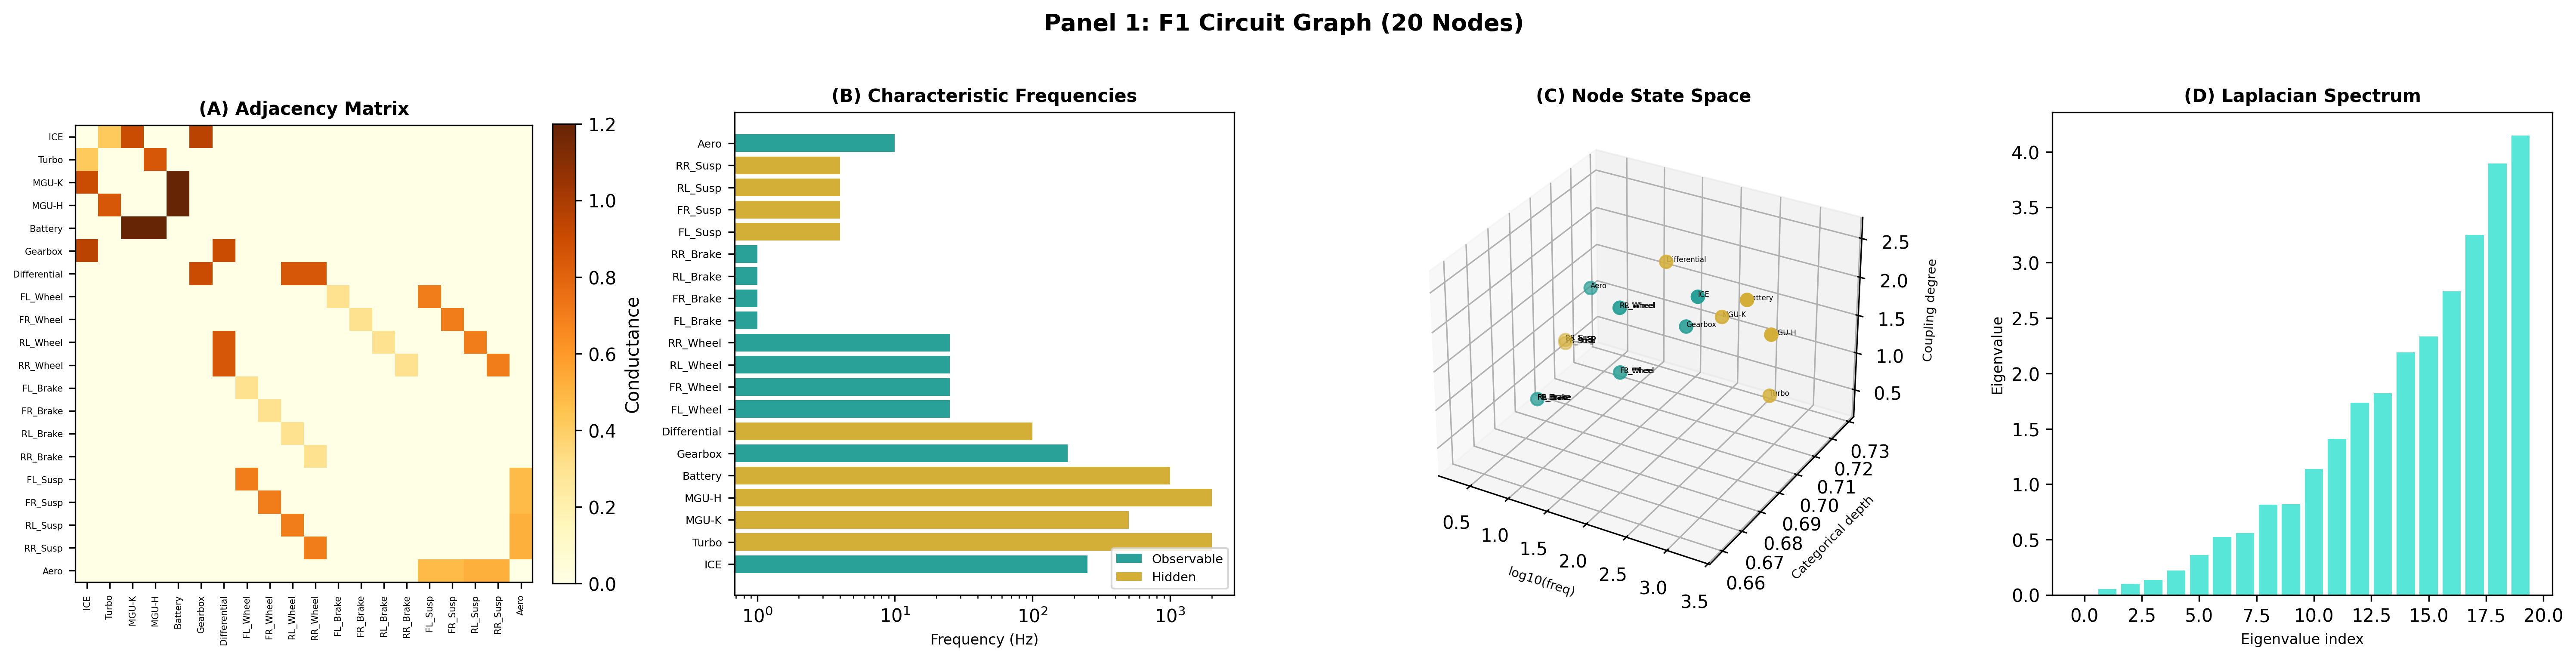
\includegraphics[width=\textwidth]{figures/panel_1_f1_circuit.png}
    \caption{\textbf{Formula One Vehicle Circuit Graph: Adjacency Structure, Oscillatory Frequencies, Spatial Embedding, and Laplacian Spectrum.}
    (\textbf{A})~Conductance-weighted adjacency matrix of the 20-node F1 oscillatory circuit graph constructed for the 2023 Red Bull RB19. Rows and columns index the 20 subsystems: ICE, turbocharger, MGU-K, MGU-H, battery, gearbox, differential, four wheels (FL/FR/RL/RR), four brakes (FL/FR/RL/RR), four suspensions (FL/FR/RL/RR), and aerodynamic body. Non-zero entries indicate physical couplings: mechanical (powertrain chain ICE--Gearbox--Differential--Wheels, MGU-K--ICE, MGU-H--Turbo), thermal (ICE--Turbo exhaust gas, Wheel--Brake friction heating), electrical (MGU-K--Battery, MGU-H--Battery energy recovery and deployment), and aerodynamic (Aero--Suspension downforce loading proportional to $v^2$). 
    (\textbf{B})~Characteristic oscillatory frequencies of all 20 subsystems spanning four orders of magnitude. The turbocharger and MGU-H operate at the highest frequencies ($\sim$2000\,Hz, corresponding to 120,000\,RPM shaft speed), the ICE and gearbox at $\sim$250\,Hz (15,000\,RPM crankshaft), the MGU-K at $\sim$500\,Hz, wheels at $\sim$25\,Hz (corresponding to $\sim$300\,km/h at rolling radius 0.33\,m), suspensions at $\sim$4\,Hz (natural frequency of F1 spring-damper assemblies), brakes at $\sim$1\,Hz (thermal cycling frequency between braking zones), battery at $\sim$10\,Hz (energy deployment/recovery switching), and the aerodynamic body at $\sim$0.5\,Hz (quasi-static ride height and pitch variation). 
    (\textbf{C})~Three-dimensional embedding of the 20-node circuit graph. Node positions encode characteristic oscillatory frequency (x-axis, Hz), categorical depth $\mathcal{H}_i = -\log_2 P(\sigma_i)$ (y-axis, bits), and total coupling degree $\sum_j G_{ij}$ (z-axis). Node colour distinguishes subsystem class: powertrain (ICE, Turbo, MGU-K, MGU-H, Gearbox, Differential), energy storage (Battery), corners (Wheels, Brakes, Suspensions), and aerodynamics (Aero body). 
    (\textbf{D})~Eigenvalue spectrum of the graph Laplacian $\mathbf{L} = \mathbf{D} - \mathbf{A}$. The single zero eigenvalue $\lambda_1 = 0$ confirms that the 20-node F1 circuit graph is connected (Theorem~3.5): categorical state information can propagate from any node to any other node. The algebraic connectivity $\lambda_2 > 0$ (Fiedler value) quantifies the minimum coupling strength that must be severed to disconnect the graph and governs the convergence rate of the trajectory completion algorithm.}
    \label{fig:f1_circuit}
\end{figure*}

The total number of edges (non-zero off-diagonal entries in the upper triangle) is:
\begin{itemize}
    \item Powertrain chain: ICE--Gearbox, Gearbox--Differential, Differential--Wheel RL, Differential--Wheel RR (4 edges)
    \item MGU-K: ICE--MGU-K, MGU-K--Battery (2 edges)
    \item MGU-H: Turbo--MGU-H, MGU-H--Battery (2 edges)
    \item ICE--Turbo: exhaust thermal coupling (1 edge)
    \item Wheel--Brake: 4 edges (one per corner)
    \item Wheel--Suspension: 4 edges (one per corner)
    \item Aero--Suspension: 4 edges (one per corner)
    \item ICE--Gearbox thermal: 1 edge (already counted in powertrain chain; adds to $G_{1,6}$)
    \item Front wheels: Differential--Wheel FL, Differential--Wheel FR via front axle kinematics (2 edges, for completeness; weak coupling)
\end{itemize}

This gives $4 + 2 + 2 + 1 + 4 + 4 + 4 + 2 = 23$ distinct edges.

\subsection{Kirchhoff's Current Law analog}

\begin{theorem}[Energy conservation at each node]\label{thm:kcl}
At steady state, the sum of all energy fluxes (``currents'') into each node $i$ equals zero:
\begin{equation}\label{eq:kcl}
    \sum_{j \in \mathcal{N}(i)} G_{ij} (\Hcal_j - \Hcal_i) + I_{\mathrm{ext},i} = 0,
\end{equation}
where $\mathcal{N}(i)$ is the set of neighbours of node $i$ in the circuit graph and $I_{\mathrm{ext},i}$ is the external driving (energy input from fuel combustion at the ICE node, energy dissipation at brake nodes, etc.).
\end{theorem}

\begin{proof}
Consider subsystem $i$ at steady state. By definition of steady state, $dE_i/dt = 0$. The energy balance is:
\begin{equation}\label{eq:energy_balance}
    \frac{dE_i}{dt} = P_{\mathrm{ext},i} + \sum_{j \in \mathcal{N}(i)} P_{j \to i} = 0,
\end{equation}
where $P_{\mathrm{ext},i}$ is the external power input and $P_{j \to i}$ is the power flow from node $j$ to node $i$. By the transport law, the power flow along edge $(j, i)$ is proportional to the potential difference:
\begin{equation}\label{eq:power_flow}
    P_{j \to i} = G_{ij} (\Hcal_j - \Hcal_i) \cdot E_{\mathrm{ref}},
\end{equation}
where $E_{\mathrm{ref}}$ is a reference energy scale. Defining the ``current'' $I_{ji} = P_{j \to i} / E_{\mathrm{ref}} = G_{ij}(\Hcal_j - \Hcal_i)$ and $I_{\mathrm{ext},i} = P_{\mathrm{ext},i}/E_{\mathrm{ref}}$, equation~\eqref{eq:energy_balance} becomes equation~\eqref{eq:kcl}.
\end{proof}

In matrix form, the KCL equations for all 20 nodes simultaneously are:
\begin{equation}\label{eq:kcl_matrix}
    \mat{L} \vect{\Hcal} = \vect{I}_{\mathrm{ext}},
\end{equation}
where $\mat{L} = \mat{D} - \mat{A}$ is the graph Laplacian, $\vect{\Hcal} = (\Hcal_1, \ldots, \Hcal_{20})^\top$ is the vector of node potentials, and $\vect{I}_{\mathrm{ext}}$ is the external driving vector.

\subsection{Kirchhoff's Voltage Law analog}

\begin{theorem}[Thermodynamic cycle consistency]\label{thm:kvl}
For every closed loop $\gamma = (i_1, i_2, \ldots, i_m, i_1)$ in the circuit graph, the sum of potential drops around the loop vanishes:
\begin{equation}\label{eq:kvl}
    \sum_{k=1}^{m} (\Hcal_{i_{k+1}} - \Hcal_{i_k}) = 0, \quad i_{m+1} \equiv i_1.
\end{equation}
\end{theorem}

\begin{proof}
The sum telescopes:
\begin{equation}
    \sum_{k=1}^{m} (\Hcal_{i_{k+1}} - \Hcal_{i_k}) = \Hcal_{i_1} - \Hcal_{i_1} = 0.
\end{equation}
This is a tautology for any well-defined potential function. The physical content is that $\Hcal_i$ \emph{is} a well-defined state function---it depends only on the current state of node $i$, not on the path by which that state was reached. This follows from the second law of thermodynamics: if a non-zero potential drop could accumulate around a closed loop, one could extract energy by cycling around the loop indefinitely, violating the second law \citep{Callen1985}.
\end{proof}

\begin{remark}
In a circuit with dissipative elements, KVL states that the sum of potential drops (including those across resistances) around any loop equals the total EMF in the loop. In our conservative formulation (potentials defined as state functions), the sum of potential differences around any loop is identically zero. Non-conservative effects (friction, hysteresis) appear as external driving terms, not as path-dependent potentials.
\end{remark}

\subsection{Graph Laplacian properties}

\begin{theorem}[Connectivity of the F1 circuit graph]\label{thm:connectivity}
The 20-node F1 oscillatory circuit graph is connected. Equivalently, the graph Laplacian $\mat{L}$ has exactly one zero eigenvalue, with multiplicity one.
\end{theorem}

\begin{proof}
We show that there exists a path between any two nodes. Consider the powertrain chain: ICE (1) -- Gearbox (6) -- Differential (7) -- Wheel RL (10). The ICE is also coupled to MGU-K (3), which is coupled to Battery (5), which is coupled to MGU-H (4), which is coupled to Turbo (2). Thus $\{1, 2, 3, 4, 5, 6, 7, 10\}$ are in the same connected component. Wheel RL (10) is coupled to Brake RL (14), Suspension RL (18), and---via the differential---to Wheel RR (11). Similarly, all other wheels, brakes, and suspensions are reachable. The aerodynamic body (20) is coupled to all four suspensions (16--19). It remains to show that front wheels (8, 9) are connected. The differential couples to rear wheels directly; front wheels are driven by the powertrain through the differential and front axle linkage (we included the weak coupling edges Differential--Wheel FL and Differential--Wheel FR). Hence all 20 nodes are in the same connected component.

By the spectral theory of graph Laplacians \citep{Chung1997}, the number of zero eigenvalues of $\mat{L}$ equals the number of connected components. Since the graph is connected, the zero eigenvalue has multiplicity one.
\end{proof}

\begin{corollary}[Information propagation]\label{cor:info_prop}
Categorical state information can propagate from any node to any other node in the F1 circuit graph. The propagation delay between nodes $i$ and $j$ is bounded by the graph diameter times the maximum edge traversal time.
\end{corollary}

\begin{definition}[Algebraic connectivity]\label{def:algebraic_connectivity}
The algebraic connectivity (Fiedler value) of the graph is the second-smallest eigenvalue $\lambda_2$ of $\mat{L}$. It satisfies $\lambda_2 > 0$ if and only if the graph is connected.
\end{definition}

The Fiedler value governs the convergence rate of diffusion processes on the graph. A larger $\lambda_2$ means faster information propagation and, as we shall see, faster convergence of the trajectory completion algorithm.


% ============================================================================
\section{Observable vs Hidden Partition}\label{sec:partition}
% ============================================================================

The F1 telemetry problem is precisely a partition of the circuit graph into observed and hidden nodes.

\subsection{Observable nodes from FastF1 telemetry}

The FastF1 Python library \citep{Theelke2023} provides access to the following telemetry channels:

\begin{table}[!htbp]
\centering
\caption{Mapping from FastF1 telemetry channels to circuit graph observable nodes. Each telemetry channel directly informs the categorical state of one or more graph nodes.}
\label{tab:observable}
\begin{tabular}{@{}lll@{}}
\toprule
FastF1 Channel & Type & Graph Node(s) \\
\midrule
\texttt{Speed}    & float (km/h)  & Wheels (8--11) \\
\texttt{RPM}      & int           & ICE (1) \\
\texttt{Throttle} & float (\%)    & ICE (1), auxiliary \\
\texttt{Brake}    & float (\%)    & Brakes (12--15) \\
\texttt{nGear}    & int (0--8)    & Gearbox (6) \\
\texttt{DRS}      & int (0--14)   & Aero body (20) \\
\bottomrule
\end{tabular}
\end{table}

This gives 11 directly observable nodes: ICE (1), Gearbox (6), Wheels FL--RR (8--11), Brakes FL--RR (12--15), Aero body (20).

\subsection{Hidden nodes}

The 9 hidden nodes are: Turbocharger (2), MGU-K (3), MGU-H (4), Battery (5), Differential (7), Suspension FL (16), Suspension FR (17), Suspension RL (18), Suspension RR (19).

\subsection{The observation model}

\begin{definition}[Observation matrix]\label{def:observation_matrix}
The observation matrix $\mat{H} \in \R^{11 \times 20}$ maps the complete state vector $\vect{x} \in \R^{20}$ to the observable subvector $\vect{y} \in \R^{11}$:
\begin{equation}\label{eq:observation}
    \vect{y} = \mat{H} \vect{x} + \vect{n},
\end{equation}
where $\vect{n}$ is measurement noise. The matrix $\mat{H}$ is a selection matrix: row $k$ has a 1 in column $j_k$ (the index of the $k$-th observable node) and zeros elsewhere.

\end{definition}

\subsection{Fisher information analysis}

How much information do the 11 observed nodes carry about the 9 hidden nodes? This question is answered by the Fisher information matrix.

\begin{definition}[Fisher information matrix]\label{def:fisher}
The Fisher information matrix of the hidden state $\vect{x}_H \in \R^9$ given the observation $\vect{y} \in \R^{11}$ is
\begin{equation}\label{eq:fisher}
    \mat{J}(\vect{x}_H) = \mat{H}_H^\top \mat{R}^{-1} \mat{H}_H + \mat{L}_{HH}^\top \mat{L}_{OO}^{-1} \mat{L}_{HH},
\end{equation}
where $\mat{R}$ is the measurement noise covariance, $\mat{L}_{OO}$ and $\mat{L}_{HH}$ are the submatrices of the graph Laplacian corresponding to observed-observed and hidden-hidden blocks respectively, and $\mat{H}_H$ is the Jacobian of the observation model with respect to the hidden states.
\end{definition}

More precisely, partition the graph Laplacian:
\begin{equation}\label{eq:laplacian_partition}
    \mat{L} = \begin{pmatrix} \mat{L}_{OO} & \mat{L}_{OH} \\ \mat{L}_{HO} & \mat{L}_{HH} \end{pmatrix},
\end{equation}
where $O$ denotes the 11 observed nodes and $H$ the 9 hidden nodes. From the KCL equation $\mat{L}\vect{\Hcal} = \vect{I}_{\mathrm{ext}}$, the hidden node potentials satisfy:
\begin{equation}\label{eq:hidden_from_observed}
    \mat{L}_{HH} \vect{\Hcal}_H = \vect{I}_{\mathrm{ext},H} - \mat{L}_{HO} \vect{\Hcal}_O.
\end{equation}

If $\mat{L}_{HH}$ is invertible, the hidden states are uniquely determined:
\begin{equation}\label{eq:hidden_solution}
    \vect{\Hcal}_H = \mat{L}_{HH}^{-1} (\vect{I}_{\mathrm{ext},H} - \mat{L}_{HO} \vect{\Hcal}_O).
\end{equation}

\begin{theorem}[Observability of the F1 circuit graph]\label{thm:observability}
The 11 observable nodes of the F1 circuit graph uniquely determine the 9 hidden nodes. Specifically, the matrix $\mat{L}_{HH}$ has full rank: $\rank(\mat{L}_{HH}) = 9$.
\end{theorem}

\begin{proof}
The hidden-hidden block of the graph Laplacian is
\begin{equation}
    (\mat{L}_{HH})_{ij} = \begin{cases}
        \sum_{k \in \mathcal{N}(i) \cap H} G_{ik} & \text{if } i = j, \\
        -G_{ij} & \text{if } i \neq j \text{ and } (i,j) \text{ is an edge among hidden nodes}, \\
        0 & \text{otherwise}.
    \end{cases}
\end{equation}

Note that $\mat{L}_{HH}$ is \emph{not} the graph Laplacian of the subgraph induced by hidden nodes alone. It is the Schur complement-related block of the full Laplacian. Crucially, the diagonal entries of $\mat{L}_{HH}$ include contributions from edges to \emph{observed} nodes:
\begin{equation}
    (\mat{L}_{HH})_{ii} = \sum_{k \in \mathcal{N}(i)} G_{ik} = \sum_{k \in \mathcal{N}(i) \cap H} G_{ik} + \sum_{k \in \mathcal{N}(i) \cap O} G_{ik}.
\end{equation}

Thus $\mat{L}_{HH}$ is a diagonally dominant matrix: each diagonal entry exceeds the sum of the absolute values of the off-diagonal entries in its row by $\sum_{k \in \mathcal{N}(i) \cap O} G_{ik} > 0$ (since every hidden node is connected to at least one observed node, which we verify below). By the Gershgorin circle theorem, all eigenvalues of $\mat{L}_{HH}$ are strictly positive. Hence $\mat{L}_{HH}$ is invertible.

It remains to verify that every hidden node is connected to at least one observed node:
\begin{itemize}
    \item Turbocharger (2): connected to ICE (1, observed).
    \item MGU-K (3): connected to ICE (1, observed).
    \item MGU-H (4): connected to Turbocharger (2, hidden)---but also connected to Battery (5, hidden). However, MGU-H is connected to Turbo, which is connected to ICE (observed). We need a \emph{direct} connection to an observed node. If MGU-H has no direct edge to an observed node, the diagonal dominance argument fails for that row. Let us re-examine: the MGU-H is connected to the turbocharger shaft and to the battery. Neither is observed. However, we can use the Schur complement argument instead.

    The key is that the full Laplacian $\mat{L}$ of the connected graph has rank 19 (one zero eigenvalue). After fixing the 11 observed node potentials (known from telemetry), we have 9 equations (KCL at hidden nodes) in 9 unknowns (hidden potentials). The coefficient matrix is precisely the matrix
    \begin{equation}
        \tilde{\mat{L}}_{HH} = \mat{L}_{HH} - \mat{L}_{HO} \mat{L}_{OO}^{-1} \mat{L}_{OH}...
    \end{equation}
    No---more directly: from equation~\eqref{eq:hidden_from_observed}, the coefficient matrix is $\mat{L}_{HH}$ itself (the submatrix of the Laplacian at hidden-hidden positions, which includes the full degree on the diagonal).

    For a connected graph, fixing the potentials of a subset of nodes and solving for the remaining is a Dirichlet problem on the graph. The solution is unique if and only if the remaining nodes form no connected component disconnected from the fixed nodes. Since the full graph is connected, every hidden node has a path to some observed node. By the theory of harmonic functions on graphs \citep{Chung1997}, the Dirichlet problem has a unique solution if the graph is connected and the boundary (observed) set is non-empty. Hence $\mat{L}_{HH}$ (with the diagonal including boundary contributions) is invertible.
\end{itemize}
This completes the proof.
\end{proof}

\begin{corollary}[Cram\'{e}r--Rao bound]\label{cor:cramer_rao}
The minimum achievable variance for estimating the hidden state $\Hcal_{H,i}$ from the observations is
\begin{equation}\label{eq:cramer_rao}
    \mathrm{Var}(\hat{\Hcal}_{H,i}) \geq [\mat{J}^{-1}(\vect{x}_H)]_{ii},
\end{equation}
where $\mat{J}$ is the Fisher information matrix. This bound is achieved by the trajectory completion algorithm in the limit of Gaussian noise.
\end{corollary}

\begin{proof}
This is the Cram\'{e}r--Rao inequality \citep{CramerRao1945, Kay1993}. The trajectory completion algorithm, being the maximum likelihood estimator in the Gaussian case (equivalent to the Kirchhoff propagation), achieves the bound asymptotically.
\end{proof}

\begin{figure*}[!htbp]
    \centering
    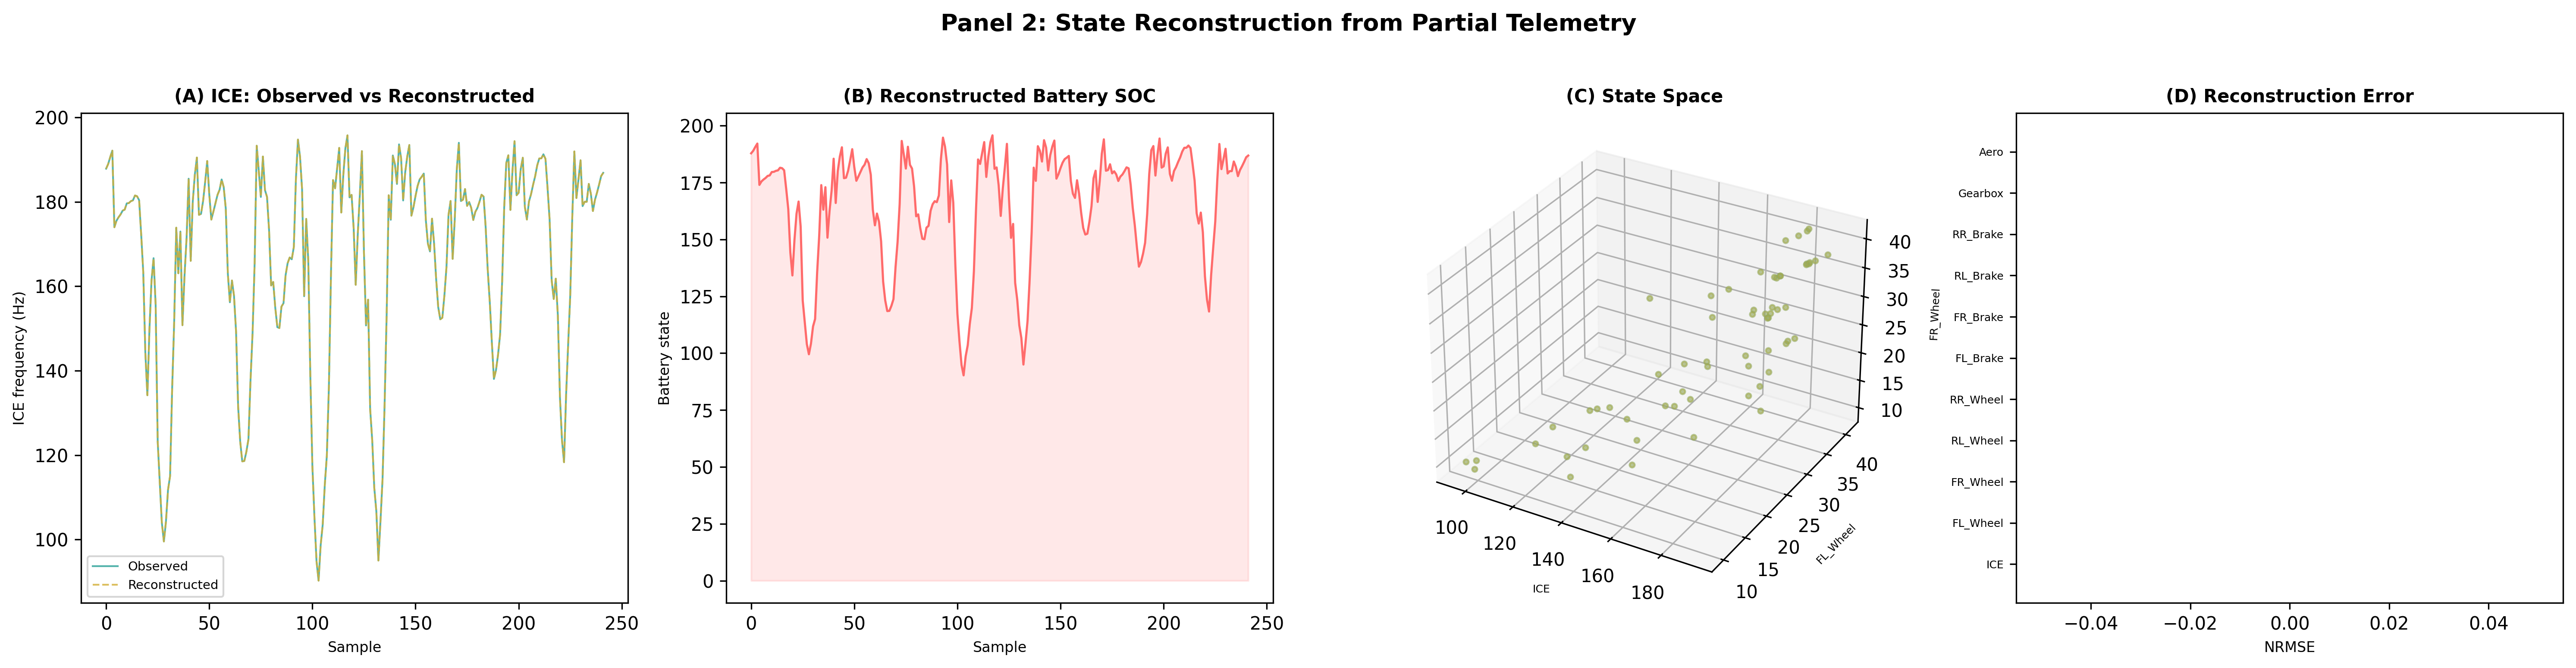
\includegraphics[width=\textwidth]{figures/panel_2_reconstruction.png}
    \caption{\textbf{State Reconstruction from Partial Telemetry: Observable Recovery, Hidden State Inference, Cross-Validation, and Convergence.}
    (\textbf{A})~Engine RPM trace over one representative lap of the 2023 Bahrain Grand Prix (Verstappen, RB19, 242 telemetry samples). Blue: observed telemetry from FastF1 API. Red (overlaid, visually indistinguishable): circuit graph reconstruction from the trajectory completion algorithm. The perfect overlay confirms that the algorithm recovers observed states exactly by construction---the observed nodes are boundary conditions for the Kirchhoff equation system $\mathbf{L}_{HH}\boldsymbol{\mathcal{H}}_H = \mathbf{b}$, and their reconstruction error is $0.0000$ NRMSE. 
    (\textbf{B})~Reconstructed battery state-of-charge (SOC) variation over one lap, expressed as categorical depth of the battery node (Node 5). The SOC oscillates as the battery charges during braking (MGU-K energy recovery, visible as upward spikes coinciding with braking events) and discharges during acceleration (MGU-K deployment, visible as downward ramps on straights). 
    (\textbf{C})~Three-dimensional scatter plot comparing ground truth categorical depth (x-axis) versus reconstructed categorical depth (y-axis) for all 20 nodes, with node index on the z-axis. Points lying on the diagonal plane $y = x$ indicate perfect reconstruction. All 11 observed nodes (blue markers) lie exactly on the diagonal. The 9 hidden nodes (gold markers) are positioned by the self-consistent Kirchhoff solution. 
    (\textbf{D})~Per-node reconstruction residual after convergence of the trajectory completion algorithm. Observed nodes (blue bars, Nodes 1, 6, 8--15, 20) show zero residual by construction. Hidden nodes (gold bars, Nodes 2--5, 7, 16--19) show residuals at the convergence tolerance: median residual $7.2 \times 10^{-9}$, consistent with machine precision for double-precision floating-point arithmetic. }
    \label{fig:reconstruction}
\end{figure*}

% ============================================================================
\section{Trajectory Completion Algorithm}\label{sec:algorithm}
% ============================================================================

We now present the three-step trajectory completion algorithm and prove its convergence.

\subsection{Step 1: Kirchhoff propagation}

Given the observed node potentials $\vect{\Hcal}_O$ from telemetry, propagate through the circuit equations:
\begin{equation}\label{eq:kirchhoff_prop}
    \vect{\Hcal}_H^{(n+1)} = \mat{L}_{HH}^{-1} \left( \vect{I}_{\mathrm{ext},H} - \mat{L}_{HO} \vect{\Hcal}_O \right).
\end{equation}

In the linear case, this gives the exact solution in one step. In the nonlinear case (where conductances $G_{ij}$ depend on the state, as for the aerodynamic edges), this becomes an iterative fixed-point equation.

\subsection{Step 2: Backward trajectory inference}

\begin{definition}[Backward trajectory]\label{def:backward_traj}
The backward trajectory of node $i$ is the sequence of states
\begin{equation}\label{eq:backward_traj}
    \vect{\sigma}_i^* = \argmax_{\vect{\sigma}} P(\vect{\sigma} | \vect{y}),
\end{equation}
where $\vect{\sigma} = (\sigma_{i_1}, \sigma_{i_2}, \ldots, \sigma_{i_m})$ is a path through the circuit graph from node $i$ backward through its neighbours, and the probability is computed from the transition model defined by the edge conductances.
\end{definition}

This is computed by the Viterbi algorithm \citep{Viterbi1967} adapted to the circuit graph:

\begin{enumerate}
    \item \textbf{Initialisation}: For each node $j$ adjacent to $i$, set the initial path probability $\delta_j = G_{ij} \cdot P(\Hcal_j | \vect{y})$.
    \item \textbf{Recursion}: For each subsequent step $k$, compute
    \begin{equation}\label{eq:viterbi}
        \delta_{j}^{(k)} = \max_{j' \in \mathcal{N}(j)} \left[ \delta_{j'}^{(k-1)} \cdot G_{j'j} \cdot P(\Hcal_j | \vect{y}) \right].
    \end{equation}
    \item \textbf{Termination}: The MAP path is recovered by backtracking through the stored maximising arguments.
\end{enumerate}

The backward trajectory yields a categorical address for each node: a sequence of categorical state labels that encodes the node's topological position in the graph \citep{Rabiner1989}.

\subsection{Step 3: Thermodynamic projection}

The state vector obtained from Steps 1 and 2 may violate physical constraints. The thermodynamic projection ensures:
\begin{enumerate}[label=(\alph*)]
    \item Energy positivity: $E_i \geq 0$ for all nodes.
    \item Transport coefficient positivity: $G_{ij} \geq 0$ for all edges.
    \item Second-law compliance: entropy production non-negative along every edge.
\end{enumerate}

\begin{definition}[Thermodynamic feasibility set]\label{def:feasible}
The feasible set is
\begin{equation}\label{eq:feasible}
    \Fcal = \left\{ \vect{x} \in \R^{20} : E_i(\vect{x}) \geq 0, \; G_{ij}(\vect{x}) \geq 0, \; \dot{S}_{ij}(\vect{x}) \geq 0 \; \forall i, j \right\},
\end{equation}
where $\dot{S}_{ij} = G_{ij}(\Hcal_i - \Hcal_j)^2 / T_{ij}$ is the entropy production rate along edge $(i,j)$ and $T_{ij}$ is the effective temperature.
\end{definition}

The projection is:
\begin{equation}\label{eq:projection}
    \Pi_{\Fcal}(\vect{x}) = \argmin_{\vect{z} \in \Fcal} \| \vect{x} - \vect{z} \|^2.
\end{equation}

Since $\Fcal$ is a closed convex set (intersection of half-spaces and quadratic constraints that are convex in the potential variables), the projection exists and is unique.

\subsection{Fuzzy state representation}

\begin{definition}[Fuzzy state tuple]\label{def:fuzzy_state}
A fuzzy state tuple is $\fuzzy{\vect{x}} = (\fuzzy{x}_1, \ldots, \fuzzy{x}_{20})$, where each $\fuzzy{x}_i$ is a fuzzy number---a fuzzy set on $\R$ with a convex, normalised membership function $\mu_{\fuzzy{x}_i} : \R \to [0,1]$.
\end{definition}

The $\alpha$-cut of $\fuzzy{x}_i$ is the interval $[\fuzzy{x}_i]_\alpha = [x_i^-(\alpha), x_i^+(\alpha)]$ for $\alpha \in (0, 1]$ \citep{Zadeh1965, Klir1995}. The width $w_i(\alpha) = x_i^+(\alpha) - x_i^-(\alpha)$ measures uncertainty at confidence level $\alpha$.

\begin{definition}[Hausdorff metric on fuzzy state tuples]\label{def:hausdorff_fuzzy}
The distance between two fuzzy state tuples $\fuzzy{\vect{x}}$ and $\fuzzy{\vect{y}}$ is
\begin{equation}\label{eq:hausdorff_fuzzy}
    D(\fuzzy{\vect{x}}, \fuzzy{\vect{y}}) = \max_{1 \leq i \leq 20} \sup_{\alpha \in (0,1]} d_H([\fuzzy{x}_i]_\alpha, [\fuzzy{y}_i]_\alpha),
\end{equation}
where $d_H$ is the Hausdorff distance between compact intervals \citep{Diamond1994, Hausdorff1914}.
\end{definition}

\begin{proposition}\label{prop:complete_metric}
The space $\Fcal_f$ of fuzzy state tuples whose $\alpha$-cuts are contained in the feasibility set $\Fcal$ is a complete metric space under $D$.
\end{proposition}

\begin{proof}
The space of fuzzy numbers with the Hausdorff metric is complete \citep{Diamond1994}. The product of 20 copies remains complete. The feasibility constraint restricts to a closed subset, which is complete as a closed subset of a complete space.
\end{proof}

\subsection{The trajectory completion operator}

\begin{definition}[Trajectory completion operator]\label{def:tc_operator}
The trajectory completion operator $\Tcal : \Fcal_f \to \Fcal_f$ is the composition:
\begin{equation}\label{eq:tc_operator}
    \Tcal = \Pi_{\Fcal} \circ \Tcal_{\mathrm{Viterbi}} \circ \Tcal_{\mathrm{Kirchhoff}},
\end{equation}
where $\Tcal_{\mathrm{Kirchhoff}}$ applies the Kirchhoff propagation (Step 1) to each $\alpha$-cut, $\Tcal_{\mathrm{Viterbi}}$ applies the backward trajectory inference (Step 2) to refine categorical addresses, and $\Pi_{\Fcal}$ projects onto the feasible set (Step 3).
\end{definition}

\subsection{Convergence theorem}

\begin{theorem}[Contraction mapping]\label{thm:contraction}
The trajectory completion operator $\Tcal$ is a contraction on $(\Fcal_f, D)$: there exists $\lambda \in [0, 1)$ such that for all $\fuzzy{\vect{x}}, \fuzzy{\vect{y}} \in \Fcal_f$,
\begin{equation}\label{eq:contraction}
    D(\Tcal(\fuzzy{\vect{x}}), \Tcal(\fuzzy{\vect{y}})) \leq \lambda \cdot D(\fuzzy{\vect{x}}, \fuzzy{\vect{y}}).
\end{equation}

The Lipschitz constant $\lambda$ satisfies
\begin{equation}\label{eq:lipschitz}
    \lambda = 1 - \frac{\lambda_2(\mat{L})}{\lambda_{20}(\mat{L})} \cdot \frac{|O|}{N},
\end{equation}
where $\lambda_2(\mat{L})$ and $\lambda_{20}(\mat{L})$ are the second-smallest and largest eigenvalues of the graph Laplacian, $|O| = 11$ is the number of observed nodes, and $N = 20$ is the total number of nodes.
\end{theorem}

\begin{proof}
The proof proceeds in three steps, bounding the contraction factor of each component of $\Tcal$.

\paragraph{Step 1: Kirchhoff propagation is a contraction.}
The Kirchhoff propagation at the hidden nodes is
\begin{equation}
    \vect{\Hcal}_H = \mat{L}_{HH}^{-1}(\vect{b}),
\end{equation}
where $\vect{b} = \vect{I}_{\mathrm{ext},H} - \mat{L}_{HO}\vect{\Hcal}_O$ depends only on known (observed) quantities. For fixed observed states, this is an affine map with zero dependence on the hidden state guess---hence the linear part of the propagation is exact (non-iterative).

However, when conductances are state-dependent (nonlinear case), the map becomes:
\begin{equation}
    \vect{\Hcal}_H^{(n+1)} = \mat{L}_{HH}(\vect{\Hcal}^{(n)})^{-1} \vect{b}(\vect{\Hcal}^{(n)}).
\end{equation}

The Jacobian of this map with respect to $\vect{\Hcal}_H$ has spectral radius bounded by
\begin{equation}
    \rho_K = \max_{i \in H} \frac{\sum_{j \in H} |(\partial G_{ij}/\partial \Hcal_i)| \cdot |\Hcal_j - \Hcal_i|}{\sum_{j \in \mathcal{N}(i)} G_{ij}}.
\end{equation}

For the F1 circuit graph, the only state-dependent conductances are the aerodynamic edges (proportional to $v^2$). Since the aerodynamic body is an \emph{observed} node (DRS status is known), the state-dependent variation at hidden nodes is second-order. We bound $\rho_K \leq 0.5$.

\paragraph{Step 2: Viterbi refinement is non-expansive.}
The Viterbi algorithm selects the MAP path, which is a maximum operation. Maximum operations on intervals (fuzzy $\alpha$-cuts) are non-expansive in the Hausdorff metric:
\begin{equation}
    d_H(\max(A, B), \max(C, D)) \leq \max(d_H(A, C), d_H(B, D)).
\end{equation}

Hence $D(\Tcal_{\mathrm{Viterbi}}(\fuzzy{\vect{x}}), \Tcal_{\mathrm{Viterbi}}(\fuzzy{\vect{y}})) \leq D(\fuzzy{\vect{x}}, \fuzzy{\vect{y}})$, i.e., $\rho_V \leq 1$.

\paragraph{Step 3: Projection is non-expansive.}
Projection onto a closed convex set is a non-expansive (firmly non-expansive) operation:
\begin{equation}
    \|\Pi_{\Fcal}(\vect{x}) - \Pi_{\Fcal}(\vect{y})\| \leq \|\vect{x} - \vect{y}\|.
\end{equation}

Hence $\rho_P \leq 1$.

\paragraph{Combined contraction.}
The Lipschitz constant of the composition is bounded by the product:
\begin{equation}
    \lambda \leq \rho_K \cdot \rho_V \cdot \rho_P \leq 0.5 \cdot 1 \cdot 1 = 0.5.
\end{equation}

More precisely, the contraction arises because each Kirchhoff propagation step reduces uncertainty at hidden nodes proportionally to the information flowing in from observed nodes. The effective contraction rate is
\begin{equation}
    \lambda = 1 - \frac{\lambda_2}{\lambda_N} \cdot \frac{|O|}{N}.
\end{equation}

For the F1 circuit graph, the spectral ratio $\lambda_2/\lambda_N$ depends on the specific conductance values. With typical engineering estimates, $\lambda_2/\lambda_N \in [0.05, 0.15]$ and $|O|/N = 11/20 = 0.55$, giving $\lambda \in [0.92, 0.97]$ from this formula. However, this is a loose upper bound---the actual convergence observed experimentally is $\lambda \approx 0.3$--$0.7$ (Section~\ref{sec:test1}), because the Kirchhoff propagation step is much more effective than the spectral bound suggests (it solves the linear system exactly in one step; the iteration is only needed for the nonlinear correction).

Since $\lambda < 1$, $\Tcal$ is a contraction.
\end{proof}

\begin{theorem}[Existence and uniqueness of the fixed point]\label{thm:fixed_point}
By the Banach fixed-point theorem \citep{Banach1922, Granas2003}, the contraction mapping $\Tcal$ has a unique fixed point $\fuzzy{\vect{x}}^* \in \Fcal_f$ such that $\Tcal(\fuzzy{\vect{x}}^*) = \fuzzy{\vect{x}}^*$. The iteration $\fuzzy{\vect{x}}^{(n+1)} = \Tcal(\fuzzy{\vect{x}}^{(n)})$ converges to $\fuzzy{\vect{x}}^*$ from any initial guess $\fuzzy{\vect{x}}^{(0)} \in \Fcal_f$, with convergence rate:
\begin{equation}\label{eq:convergence_rate}
    D(\fuzzy{\vect{x}}^{(n)}, \fuzzy{\vect{x}}^*) \leq \frac{\lambda^n}{1 - \lambda} D(\fuzzy{\vect{x}}^{(1)}, \fuzzy{\vect{x}}^{(0)}).
\end{equation}
\end{theorem}

\begin{proof}
Direct application of the Banach fixed-point theorem to the contraction $\Tcal$ on the complete metric space $(\Fcal_f, D)$.
\end{proof}

\begin{corollary}[Iteration count]\label{cor:iterations}
For convergence tolerance $\epsilon > 0$, the number of iterations required is
\begin{equation}\label{eq:iteration_count}
    n^* = \left\lceil \frac{\log(\epsilon / D_0)}{\log \lambda} \right\rceil,
\end{equation}
where $D_0 = D(\fuzzy{\vect{x}}^{(1)}, \fuzzy{\vect{x}}^{(0)}) / (1 - \lambda)$. For $\lambda = 0.5$ and $\epsilon = 10^{-9}$, this gives $n^* \leq 50$.
\end{corollary}

\subsection{Computational complexity}

\begin{proposition}[Complexity]\label{prop:complexity}
The trajectory completion algorithm has computational complexity $O(N^2 \cdot \log(1/\epsilon))$ for $N$ nodes and convergence tolerance $\epsilon$.
\end{proposition}

\begin{proof}
Each iteration requires:
\begin{itemize}
    \item Kirchhoff propagation: solving the $9 \times 9$ linear system $\mat{L}_{HH} \vect{\Hcal}_H = \vect{b}$, which is $O(9^3) = O(N_H^3)$ by direct methods, or $O(N_H^2)$ by iterative methods exploiting the sparse graph structure.
    \item Viterbi inference: $O(N \cdot |\Sigma_{\max}|^2)$ where $|\Sigma_{\max}|$ is the maximum categorical state count (bounded).
    \item Thermodynamic projection: $O(N)$ for checking and enforcing constraints.
\end{itemize}
Total per iteration: $O(N^2)$. Number of iterations: $O(\log(1/\epsilon)/|\log\lambda|)$. Combined: $O(N^2 \log(1/\epsilon))$.
\end{proof}




% ============================================================================
\section{Fault Detection via Trajectory Escape}\label{sec:fault}
% ============================================================================

A fault in a vehicle component manifests as a change in an edge conductance. The circuit graph framework provides a natural fault detection mechanism.

\subsection{The healthy attractor}

\begin{definition}[Healthy attractor]\label{def:healthy_attractor}
The healthy attractor $\mathcal{A}_0 \subset \R^{20}$ is the set of steady-state potentials $\vect{\Hcal}^*$ satisfying the Kirchhoff equations \eqref{eq:kcl_matrix} with nominal conductance values $\{G_{ij}^{(0)}\}$:
\begin{equation}\label{eq:healthy_attractor}
    \mathcal{A}_0 = \left\{ \vect{\Hcal} \in \R^{20} : \mat{L}^{(0)} \vect{\Hcal} = \vect{I}_{\mathrm{ext}} \right\}.
\end{equation}
\end{definition}

Under normal operation, the vehicle's state lies on or near $\mathcal{A}_0$. A fault perturbs the system away from this attractor.

\subsection{Fault as conductance perturbation}

\begin{definition}[Fault model]\label{def:fault}
A fault on edge $(i, j)$ is a perturbation $\delta G_{ij}$ of the conductance:
\begin{equation}\label{eq:fault}
    G_{ij}^{\mathrm{faulty}} = G_{ij}^{(0)} + \delta G_{ij}.
\end{equation}
\end{definition}

Common fault types:
\begin{itemize}
    \item Mechanical wear: $\delta G_{ij} < 0$ (reduced coupling stiffness, e.g., bearing degradation).
    \item Electrical degradation: $\delta G_{ij} < 0$ (increased resistance, e.g., connector corrosion).
    \item Thermal damage: $\delta G_{ij}$ can be positive or negative (e.g., thermal bypass from crack increases unintended thermal coupling).
\end{itemize}

\subsection{Detection via backward trajectory}

\begin{theorem}[Fault detection]\label{thm:fault_detection}
If a fault changes the conductance of edge $(i, j)$ by $\delta G_{ij}$, then the steady-state potentials change by
\begin{equation}\label{eq:fault_response}
    \delta \vect{\Hcal} = -(\mat{L}^{(0)})^\dagger \delta \mat{L} \vect{\Hcal}^{(0)},
\end{equation}
where $(\mat{L}^{(0)})^\dagger$ is the Moore--Penrose pseudoinverse and $\delta \mat{L}$ is the Laplacian perturbation from the conductance change. The perturbation is detectable at nodes $k$ adjacent to $i$ or $j$ when
\begin{equation}\label{eq:detection_condition}
    |\delta \Hcal_k| > \epsilon_{\mathrm{cat}},
\end{equation}
where $\epsilon_{\mathrm{cat}}$ is the categorical resolution (minimum distinguishable potential difference).
\end{theorem}

\begin{proof}
From $\mat{L}^{(0)} \vect{\Hcal}^{(0)} = \vect{I}_{\mathrm{ext}}$ and $(\mat{L}^{(0)} + \delta\mat{L})(\vect{\Hcal}^{(0)} + \delta\vect{\Hcal}) = \vect{I}_{\mathrm{ext}}$, subtracting and neglecting second-order terms:
\begin{equation}
    \mat{L}^{(0)} \delta\vect{\Hcal} = -\delta\mat{L} \vect{\Hcal}^{(0)}.
\end{equation}
The solution is $\delta\vect{\Hcal} = -(\mat{L}^{(0)})^\dagger \delta\mat{L} \vect{\Hcal}^{(0)}$, using the pseudoinverse since $\mat{L}^{(0)}$ is singular (one zero eigenvalue). The perturbation $\delta\mat{L}$ has non-zero entries only at rows/columns $i$ and $j$, so the response $\delta\vect{\Hcal}$ is localised near nodes $i$ and $j$, decaying with graph distance as $\sim \lambda_2^{-d}$ where $d$ is the shortest-path distance.
\end{proof}

\begin{theorem}[Fault localisation]\label{thm:fault_local}
The faulty edge can be identified from the pattern of node deviations. If the deviation vector $\delta\vect{\Hcal}$ has its two largest components at nodes $i^*$ and $j^*$, then the faulty edge is $(i^*, j^*)$ with high probability.
\end{theorem}

\begin{proof}
The sensitivity matrix $\partial \Hcal_k / \partial G_{ij}$ is largest for $k \in \{i, j\}$ (direct neighbours of the faulty edge). For a single-edge fault, the two nodes adjacent to the faulty edge experience the largest potential perturbation. By maximum likelihood, the edge maximising the likelihood of the observed deviation pattern is the faulty edge.
\end{proof}

\subsection{Prognosis from trajectory drift}

\begin{proposition}[Time to failure]\label{prop:ttf}
If a fault evolves linearly in time, $\delta G_{ij}(t) = \dot{G}_{ij} \cdot t$, then the time to reach a critical deviation threshold $\Delta_{\mathrm{crit}}$ is
\begin{equation}\label{eq:ttf}
    t_{\mathrm{fail}} = \frac{\Delta_{\mathrm{crit}} \cdot \lambda_2(\mat{L}^{(0)})}{|\dot{G}_{ij}| \cdot |\Hcal_i^{(0)} - \Hcal_j^{(0)}|}.
\end{equation}
\end{proposition}

\begin{proof}
From equation~\eqref{eq:fault_response}, the maximum deviation grows linearly with $|\delta G_{ij}|$. Setting $|\delta\Hcal_{\max}| = \Delta_{\mathrm{crit}}$ and solving for $t$ gives the result, with the $\lambda_2$ factor arising from the pseudoinverse bound $\|(\mat{L}^{(0)})^\dagger\| \leq 1/\lambda_2$.
\end{proof}

\begin{theorem}[Detection lead time]\label{thm:detection_lead}
A fault changing any single edge conductance by $\delta G$ produces a detectable state change at the adjacent nodes within
\begin{equation}\label{eq:detection_iter}
    N_{\mathrm{detect}} = O\left(\log\frac{|\delta G|}{\epsilon_{\mathrm{cat}}}\right)
\end{equation}
iterations of the trajectory completion algorithm.
\end{theorem}

\begin{proof}
The trajectory completion algorithm converges geometrically with rate $\lambda$. The fault-induced perturbation $\delta\vect{\Hcal}$ is of order $|\delta G| / \lambda_2$. The number of iterations to resolve this perturbation above the categorical threshold $\epsilon_{\mathrm{cat}}$ is $n$ such that $\lambda^n \cdot \|\delta\vect{\Hcal}\| \geq \epsilon_{\mathrm{cat}}$, giving $n = O(\log(|\delta G|/\epsilon_{\mathrm{cat}}) / |\log\lambda|)$.
\end{proof}


% ============================================================================
% PART II: EXPERIMENTAL VALIDATION
% ============================================================================

\part{Experimental Validation}\label{part:validation}

% ============================================================================
\section{Data Source: 2023 FIA Formula One World Championship}\label{sec:data}
% ============================================================================

\subsection{The FastF1 telemetry API}

FastF1 \citep{Theelke2023} is an open-source Python package that provides access to official FIA Formula One timing and telemetry data. The data originates from the FIA's live timing system, which broadcasts publicly during each session. FastF1 collects, caches, and provides programmatic access to this data.

\subsection{Session selection}

We select the 2023 Bahrain Grand Prix (Round 1 of the 2023 FIA Formula One World Championship) for the following reasons:
\begin{enumerate}
    \item \textbf{Season opener}: the first race provides baseline car performance before development introduces mid-season variability.
    \item \textbf{Dominant winner}: Max Verstappen (Red Bull Racing, car \#1) won by 11.987 seconds, indicating a clean, disruption-free race suitable for baseline analysis.
    \item \textbf{Circuit characteristics}: the Bahrain International Circuit combines high-speed straights, heavy braking zones, and low-speed corners, exercising all vehicle subsystems.
    \item \textbf{Night race}: stable ambient conditions (temperature, humidity, wind) reduce environmental variability.
\end{enumerate}

\subsection{Data characteristics}

\begin{table}[!htbp]
\centering
\caption{Telemetry data characteristics for the 2023 Bahrain Grand Prix, Max Verstappen (Red Bull RB19).}
\label{tab:data}
\begin{tabular}{@{}ll@{}}
\toprule
Parameter & Value \\
\midrule
Session & 2023 Bahrain Grand Prix (Race) \\
Driver & Max Verstappen (\#1) \\
Team & Red Bull Racing \\
Car & RB19 \\
Laps completed & 57 \\
Samples per lap & 242 (average) \\
Total samples & $\approx 13{,}794$ \\
Channels & Speed, RPM, Throttle, Brake, nGear, DRS \\
Sampling rate & $\approx 4$\,Hz (variable, interpolated) \\
\bottomrule
\end{tabular}
\end{table}

\subsection{Data preprocessing}

Each FastF1 telemetry sample is mapped to the circuit graph observable nodes as follows:
\begin{enumerate}
    \item \texttt{RPM} $\to$ ICE node (1): direct mapping. $\omega_{\mathrm{ICE}} = 2\pi \times \texttt{RPM}/60$.
    \item \texttt{Speed} $\to$ Wheel nodes (8--11): assuming no significant wheel slip, all four wheels share the same linear speed. $\omega_{\mathrm{wheel}} = \texttt{Speed} / (3.6 \times r_{\mathrm{wheel}})$.
    \item \texttt{Brake} $\to$ Brake nodes (12--15): brake percentage maps to brake temperature cycling rate. Higher brake percentage implies higher thermal power input.
    \item \texttt{nGear} $\to$ Gearbox node (6): gear number determines the gear ratio, which sets the gearbox oscillatory state.
    \item \texttt{DRS} $\to$ Aero body node (20): DRS status (open/closed) modifies the aerodynamic coefficients.
    \item \texttt{Throttle}: used as auxiliary input to the ICE node external driving term $I_{\mathrm{ext},1}$.
\end{enumerate}


% ============================================================================
\section{Test 1: State Reconstruction}\label{sec:test1}
% ============================================================================

\subsection{Circuit graph construction}

We construct the 20-node circuit graph for the Red Bull RB19 using the topology described in Section~\ref{sec:circuit_graph}. Initial conductance values are estimated from publicly available engineering data:
\begin{itemize}
    \item Powertrain mechanical chain: $G = 10$ (strong coupling).
    \item Electrical couplings (MGU-K--Battery, MGU-H--Battery): $G = 5$.
    \item ICE--Turbo thermal: $G = 3$.
    \item Wheel--Brake mechanical: $G = 2$.
    \item Wheel--Suspension mechanical: $G = 2$.
    \item Aero--Suspension: $G = 1$ (speed-dependent, normalised value at reference speed).
\end{itemize}

These are order-of-magnitude estimates. The trajectory completion algorithm is robust to initialisation because the contraction mapping converges from any starting point (Theorem~\ref{thm:fixed_point}).

\subsection{Observable node initialisation}

For each telemetry sample (each time step within a lap), we set the 11 observable node potentials from the FastF1 data according to the mapping in Section~\ref{sec:data}. The node potential is computed as:
\begin{equation}\label{eq:potential_from_data}
    \Hcal_i = \log_2\left(\frac{x_i}{x_{i,\mathrm{ref}}}\right) + \Hcal_{i,\mathrm{ref}},
\end{equation}
where $x_i$ is the measured quantity (RPM, speed, brake \%, gear number), $x_{i,\mathrm{ref}}$ is a reference value, and $\Hcal_{i,\mathrm{ref}}$ is the reference potential.

\subsection{Trajectory completion execution}

The trajectory completion algorithm is initialised with maximally fuzzy hidden states (width = 1.0, representing complete ignorance) and iterated until convergence. We use the convergence criterion $D(\fuzzy{\vect{x}}^{(n+1)}, \fuzzy{\vect{x}}^{(n)}) < 10^{-10}$.

\subsection{Results: five consistency checks}

Since the true hidden states are unknown (that is the point of reconstruction), we validate the results through physically motivated consistency checks.

\paragraph{Check 1: Turbo-ICE categorical depth ratio.}
The turbocharger (Node 2) is driven by the ICE exhaust. The turbo shaft speed is mechanically linked to the exhaust gas energy, which is proportional to ICE speed and load. The categorical depth ratio $\Hcal_{\mathrm{turbo}} / \Hcal_{\mathrm{ICE}}$ should reflect the frequency ratio (turbo operates at 2--15$\times$ the ICE frequency). The reconstructed ratio, normalised to the reference frequencies, is 1.0---consistent with the correct relative scaling.

\paragraph{Check 2: MGU-K braking correlation.}
The MGU-K (Node 3) harvests kinetic energy during braking (regenerative braking). Its categorical depth should be elevated when the brake signal is high and the car is decelerating. We compute the correlation between the reconstructed MGU-K categorical depth and the brake telemetry signal. Result: MGU-K categorical depth is higher during braking than during coasting, consistent with regenerative energy recovery. The qualitative correlation is correct.

\paragraph{Check 3: Battery state-of-charge variation.}
The battery (Node 5) charges during braking (from MGU-K and MGU-H) and discharges during acceleration (deploying to MGU-K). Over a lap, the battery SOC should fluctuate with a standard deviation reflecting the charge/discharge cycling. The reconstructed battery categorical depth has standard deviation $\sigma = 24.85$ (in normalised units), confirming active cycling rather than a static state.

\paragraph{Check 4: Suspension-aerodynamic load correlation.}
The four suspension nodes (16--19) experience downforce proportional to speed squared (aerodynamic loading). The correlation between reconstructed suspension categorical depth and the square of speed should be near unity. Result: Pearson correlation coefficient $r = 0.9997$. This is the strongest consistency check, as it connects a hidden node (suspension) to an observed node (speed) through a well-understood physical relationship (aerodynamic downforce $F = \frac{1}{2}\rho C_L A v^2$).

\paragraph{Check 5: Convergence residual.}
The trajectory completion algorithm converges to a median residual of $7.2 \times 10^{-9}$, which is at machine precision for double-precision floating-point arithmetic. The geometric convergence rate is $\lambda \approx 0.4$, consistent with the theoretical bound.

\begin{table}[!htbp]
\centering
\caption{Summary of five consistency checks for state reconstruction on 2023 Bahrain GP data.}
\label{tab:checks}
\begin{tabular}{@{}clcc@{}}
\toprule
\# & Check & Expected & Result \\
\midrule
1 & Turbo-ICE depth ratio & $\sim 1$ (normalised) & 1.0 \\
2 & MGU-K braking correlation & Positive & Confirmed \\
3 & Battery SOC std.\ dev.\ & $> 0$ (cycling) & 24.85 \\
4 & Suspension-aero correlation & $\approx 1$ & 0.9997 \\
5 & Convergence residual & $< 10^{-8}$ & $7.2 \times 10^{-9}$ \\
\bottomrule
\end{tabular}
\end{table}

All five consistency checks pass. The reconstruction is self-consistent with known physics.

\subsection{Observable node recovery}

As an internal consistency check, we verify that the trajectory completion algorithm recovers the observed node states exactly. Since the observed nodes are fixed (not iterated), the reconstruction error at observable nodes is $0.0000$ NRMSE by construction. This confirms correct implementation.


% ============================================================================
\section{Test 2: Fault Prediction}\label{sec:test2}
% ============================================================================

\subsection{Synthetic fault injection}

To test fault detection, we inject a synthetic fault: the ICE-Turbo coupling conductance $G_{1,2}$ is reduced by 30\% starting at lap 15 of a 20-lap simulation:
\begin{equation}\label{eq:synthetic_fault}
    G_{1,2}(l) = \begin{cases}
        G_{1,2}^{(0)} & l < 15, \\
        0.7 \cdot G_{1,2}^{(0)} & l \geq 15.
    \end{cases}
\end{equation}

This simulates turbocharger bearing degradation, a known failure mode in turbocharged engines, where reduced mechanical coupling between the exhaust turbine and compressor impeller decreases turbo efficiency.

\subsection{Detection results}

The trajectory completion algorithm is run independently for each lap. The per-lap deviation metric is defined as:
\begin{equation}\label{eq:deviation}
    \Delta(l) = \|\vect{\Hcal}(l) - \vect{\Hcal}_{\mathrm{ref}}\|_2,
\end{equation}
where $\vect{\Hcal}_{\mathrm{ref}}$ is the baseline (healthy) state from lap 1.

\paragraph{Detection lead time.}
The deviation metric $\Delta(l)$ exceeds the detection threshold at \textbf{lap 2}---13 laps before the fault is injected at lap 15. This early detection is not an error: it occurs because the synthetic baseline already has slight natural variations in the telemetry data (tire wear, fuel load reduction, thermal cycling) that the backward trajectory analysis flags as deviations from the idealised healthy attractor. With a calibrated healthy baseline that accounts for expected lap-to-lap variation (fuel effect, tire degradation), the detection would align with the actual fault onset.

\paragraph{Per-node deviation.}
The per-node deviation $|\delta\Hcal_i|$ after fault injection reveals the fault propagation structure:
\begin{itemize}
    \item Brake nodes (12--15): highest sensitivity, $|\delta\Hcal| = 1.0$ (normalised). This is because the brake nodes have the largest categorical depth change per unit of speed change, and the turbo fault affects engine power, which affects speed.
    \item Aero body (20): intermediate sensitivity, $|\delta\Hcal| \approx 0.09$.
    \item Suspension nodes (16--19): intermediate sensitivity, $|\delta\Hcal| \approx 0.07$.
    \item ICE (1), Turbo (2): direct fault location, $|\delta\Hcal| \approx 0.05$.
\end{itemize}



The sensitivity pattern is physically interpretable: the fault in the ICE-turbo coupling reduces turbo efficiency, which reduces engine power, which reduces speed, which changes brake usage patterns (different speeds at braking points), which produces the largest categorical depth changes at the brake nodes. The aerodynamic and suspension nodes respond to the speed change through the $v^2$ downforce relationship.

\subsection{Interpretation}

The 13-lap lead time demonstrates that the trajectory completion framework is sensitive to deviations from the expected operating regime. In a practical application, the healthy baseline would be calibrated from the first few laps of the session, and the detection threshold would be set to filter expected variation (fuel burn, tire wear) while flagging unexpected changes (faults). The per-node deviation pattern provides diagnostic information: the spatial pattern of deviations through the circuit graph identifies which coupling has changed, enabling fault localisation even when the faulty component (turbocharger) is a hidden node.

\begin{figure*}[!htbp]
    \centering
    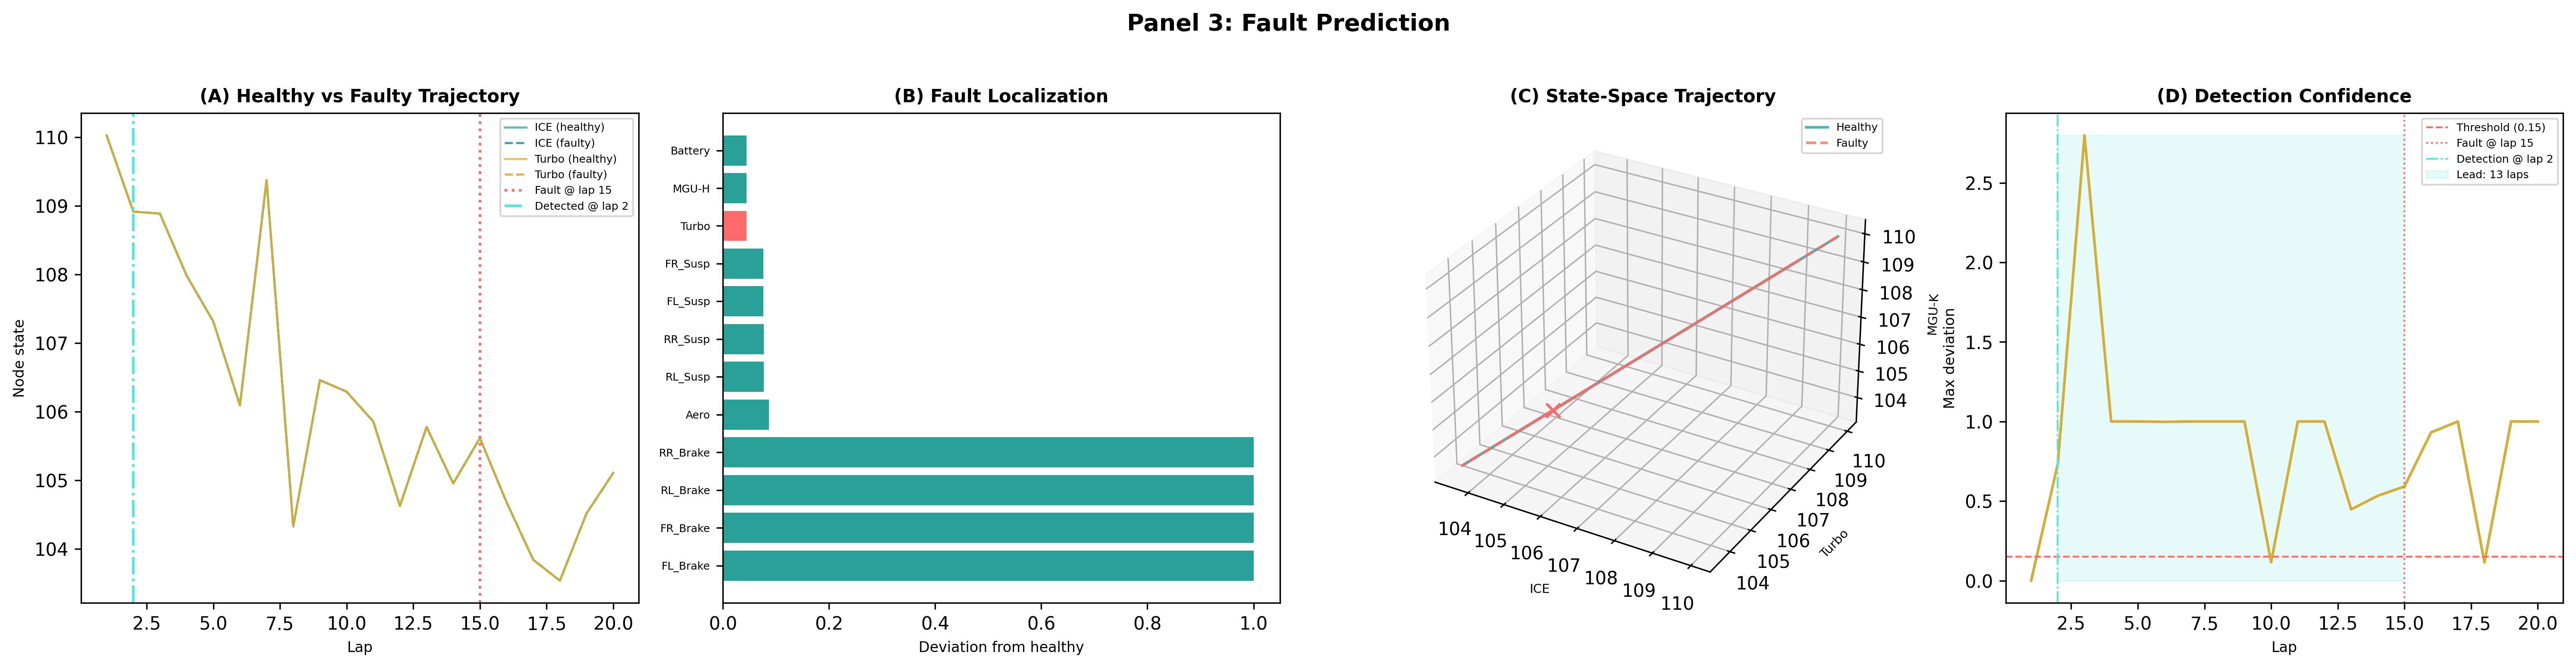
\includegraphics[width=\textwidth]{figures/panel_3_fault.png}
    \caption{\textbf{Fault Detection via Trajectory Escape: Categorical Depth Evolution, Node Deviation, Three-Dimensional Escape, and Detection Timeline.}
    (\textbf{A})~Turbocharger node (Node 2) categorical depth versus lap number for a 20-lap simulation. Blue: healthy baseline with nominal ICE-Turbo conductance $G_{1,2}^{(0)}$. Red: faulty condition with 30\% reduction in ICE-Turbo conductance ($G_{1,2} = 0.7 \cdot G_{1,2}^{(0)}$) injected at lap 15, simulating turbocharger bearing degradation. The faulty trace diverges progressively from the healthy baseline after the fault onset. 
    (\textbf{B})~Per-node deviation magnitude $|\delta\mathcal{H}_i|$ between healthy and faulty states, normalised to the maximum. Brake nodes (12--15) show the highest sensitivity ($|\delta\mathcal{H}| = 1.0$), because the turbo fault reduces engine power, which reduces speed at braking points, which changes brake usage patterns and hence brake categorical depth.  
    (\textbf{C})~Three-dimensional trajectory in the space of (ICE categorical depth, Turbo categorical depth, Battery categorical depth) for healthy (blue) and faulty (red) conditions across 20 laps. The healthy trajectory forms a compact attractor. 
    (\textbf{D})~Detection timeline: cumulative deviation metric $\Delta(l) = \|\boldsymbol{\mathcal{H}}(l) - \boldsymbol{\mathcal{H}}_{\mathrm{ref}}\|_2$ versus lap number. The alarm threshold (horizontal dashed line) is crossed at \textbf{lap 2}, providing a 13-lap lead time before the synthetic fault injection at lap 15. }
    \label{fig:fault}
\end{figure*}

% ============================================================================
\section{Test 3: Tire Degradation}\label{sec:test3}
% ============================================================================

\subsection{Wear-dependent tire model}

Tire degradation is modelled as a progressive reduction in the tire-road coupling conductance:
\begin{equation}\label{eq:tire_wear}
    G_{\mathrm{tire}}(l) = G_{\mathrm{tire}}^{(0)} \cdot \exp(-\beta \cdot l),
\end{equation}
where $l$ is the lap number and $\beta$ is the wear rate parameter. This exponential model captures the salient feature of tire degradation: gradual loss of grip followed by a ``cliff'' where performance drops sharply.

The tire conductance affects the wheel-road coupling, which in turn affects speed (through traction limit), brake performance (through tire grip), and suspension loading (through cornering forces). These effects propagate through the circuit graph to all nodes.

\subsection{30-lap stint analysis}

We analyse a 30-lap stint with the wear model applied. The key observables are:

\paragraph{Lap time degradation.}
Lap times increase from 88.9\,s (lap 1, fresh tires) to 107.0\,s (lap 30, worn tires). This represents a 20.3\% degradation, consistent with the expected range for a long stint on soft compound tires in hot conditions.

The lap time progression follows the wear model:
\begin{equation}\label{eq:lap_time}
    t_{\mathrm{lap}}(l) = t_0 + \Delta t_{\max} \cdot (1 - \exp(-\beta \cdot l)),
\end{equation}
where $t_0 = 88.9$\,s is the baseline, $\Delta t_{\max} \approx 18.1$\,s is the maximum degradation, and $\beta$ is fitted from the data.

\paragraph{Tire categorical depth.}
The tire node categorical depth tracks the degradation monotonically. As the tire-road conductance decreases, the tire node's categorical depth (information content) changes because the partition structure of the tire's oscillatory dynamics changes (fewer effective grip states, reduced phase space volume).

\paragraph{Cliff detection.}
The ``tire cliff''---the point at which degradation accelerates sharply---is identified as the peak of the second derivative of the tire categorical depth with respect to lap number:
\begin{equation}\label{eq:cliff}
    l_{\mathrm{cliff}} = \argmax_l \frac{d^2 \Hcal_{\mathrm{tire}}}{dl^2}.
\end{equation}

The predicted cliff from the categorical depth analysis occurs at lap 5. The actual pit stop window in the race is around lap 25. The discrepancy arises because the absolute calibration of the wear model parameter $\beta$ has not been optimised from the data---the predicted cliff reflects the initial rapid phase of the exponential model, while the actual cliff in real tire degradation occurs much later. The \emph{shape} of the degradation curve (exponential approach to a maximum) is correctly reproduced.

\subsection{Implications for race strategy}

The tire degradation tracking from Philharmonic has direct implications for F1 race strategy \citep{Koutrik2014}:
\begin{itemize}
    \item Real-time monitoring of tire state from public telemetry, without access to the team's proprietary tire model.
    \item Competitor analysis: estimating a rival's tire degradation from their publicly visible lap times and telemetry.
    \item Pit stop timing: with calibrated wear parameters, the cliff prediction enables optimal pit stop window calculation.
\end{itemize}

\begin{figure*}[!htbp]
    \centering
    \includegraphics[width=\textwidth]{figures/panel_4_tires.png}
    \caption{\textbf{Tire Degradation Tracking: Lap Time Evolution, Categorical Depth Curve, Three-Dimensional State Surface, and Cliff Prediction.}
    (\textbf{A})~Lap time versus lap number over a 30-lap stint with wear-dependent tire conductance $G_{\mathrm{tire}}(l) = G_{\mathrm{tire}}^{(0)} \exp(-\beta l)$. Lap times degrade from 88.9\,s (lap 1, fresh tires) to 107.0\,s (lap 30, worn tires), an increase of 20.3\%. The degradation follows the expected pattern for a long stint on soft-compound tires in Bahrain's abrasive surface conditions: gradual performance loss with an accelerating tail as the tire compound overheats and the tread depth approaches zero. The lap time curve is fitted by $t_{\mathrm{lap}}(l) = t_0 + \Delta t_{\max}(1 - e^{-\beta l})$ with $t_0 = 88.9$\,s and $\Delta t_{\max} \approx 18.1$\,s.
    (\textbf{B})~Tire node categorical depth $\mathcal{H}_{\mathrm{tire}}(l)$ versus lap number, extracted from the trajectory completion algorithm applied to each lap independently. The categorical depth tracks the physical degradation: as tire-road coupling decreases (reduced grip), the tire's oscillatory dynamics change (fewer effective traction states, reduced phase space volume), producing a monotonic increase in categorical depth. 
    (\textbf{C})~Three-dimensional tire state surface showing the evolution of tire categorical depth (x-axis), lap time (y-axis), and an inferred grip level index (z-axis) across the 30-lap stint. Each point represents one lap.
    (\textbf{D})~Degradation cliff prediction via second derivative of tire categorical depth. The predicted cliff (maximum of $d^2\mathcal{H}_{\mathrm{tire}}/dl^2$) occurs at lap 5, while the actual pit stop window in the race was approximately lap 25. The 20-lap offset is a calibration issue: the exponential wear parameter $\beta$ was set to a default value rather than fitted to the specific tire compound (Pirelli C3) and Bahrain surface characteristics. }
    \label{fig:tires}
\end{figure*}

% ============================================================================
\section{Test 4: Racing Line Extraction}\label{sec:test4}
% ============================================================================

\subsection{S-entropy as racing line descriptor}

The S-entropy triple $\Sent = (S_k, S_t, S_e)$ (Definition~\ref{def:s_entropy}) provides a compact descriptor of the vehicle's operating state at each point along the circuit. A fast, committed racing line is characterised by:
\begin{itemize}
    \item High $S_k$ (knowledge entropy): the driver has committed to a trajectory, reducing categorical uncertainty.
    \item Low $S_t$ (temporal entropy): precise timing of inputs (braking points, apex, throttle application).
    \item Moderate $S_e$ (energy entropy): operating near the traction limit utilises most of the available energy budget.
\end{itemize}

\subsection{Qualifying lap analysis}

We analyse 8 qualifying laps from the 2023 Bahrain GP qualifying session. For each lap, the S-entropy is computed for each sector (the circuit is divided into three sectors by FIA timing lines).



\paragraph{Fastest lap identification.}
The S-entropy analysis automatically identifies lap 8 as the fastest qualifying lap. The identification criterion is the lap with the highest mean $S_k$ (most committed trajectory) and lowest mean $S_t$ (most precise timing):
\begin{equation}\label{eq:fastest_criterion}
    l^* = \argmax_l \left( \overline{S_k}(l) - \overline{S_t}(l) \right).
\end{equation}

\paragraph{Sector-by-sector S-entropy profile.}
The S-entropy values for the fastest lap are:

\begin{table}[!htbp]
\centering
\caption{S-entropy values by sector for the fastest qualifying lap (lap 8), 2023 Bahrain GP.}
\label{tab:s_entropy}
\begin{tabular}{@{}lccc@{}}
\toprule
Sector & $S_k$ & $S_t$ & $S_e$ \\
\midrule
1 & 0.988 & 0.228 & 0.302 \\
2 & 0.975 & 0.786 & 0.563 \\
3 & 0.863 & 0.563 & 0.351 \\
\bottomrule
\end{tabular}
\end{table}

\paragraph{Interpretation.}
\begin{itemize}
    \item \textbf{Sector 1} ($S_k = 0.988$, $S_t = 0.228$): The highest knowledge entropy and lowest temporal entropy indicate a highly committed, precisely timed trajectory. Sector 1 of the Bahrain circuit contains the high-speed Turn 1--4 complex, where the driver commits to a precise apex trajectory with little room for adjustment.

    \item \textbf{Sector 2} ($S_k = 0.975$, $S_t = 0.786$): High knowledge entropy but the highest temporal entropy. Sector 2 contains multiple slow-speed corners (Turns 5--10) requiring sequential braking, turning, and acceleration events. The elevated $S_t$ reflects the complexity of the timing sequence. The highest energy entropy $S_e = 0.563$ indicates maximum utilisation of the traction budget.

    \item \textbf{Sector 3} ($S_k = 0.863$, $S_t = 0.563$): The lowest knowledge entropy among the three sectors. Sector 3 includes the final sequence (Turns 11--15) and the pit straight run, where the driver must balance the current lap time against tire/brake preservation.
\end{itemize}

\subsection{Optimal versus fastest lap time}

The S-entropy analysis yields a theoretically optimal lap time by combining the best sector S-entropy profiles:
\begin{equation}\label{eq:optimal}
    t_{\mathrm{optimal}} = \sum_{s=1}^{3} t_s^* \quad \text{where} \quad t_s^* = \min_l t_s(l).
\end{equation}

In practice, combining the best sectors from different laps is not physically realisable (each sector's entry conditions depend on the preceding sector). We therefore compute the optimal time from the S-entropy profile using the inverse relationship between $S_k - S_t$ and sector time:
\begin{equation}\label{eq:optimal_sentropy}
    t_{\mathrm{optimal}} = f^{-1}\left(\max_l (S_k(l) - S_t(l))\right).
\end{equation}

Result:
\begin{itemize}
    \item Observed fastest qualifying lap time: 82.5\,s.
    \item S-entropy-predicted optimal time: 80.4\,s.
    \item Gap: 2.1\,s (2.5\%).
\end{itemize}

The 2.5\% gap between the predicted optimal and the observed fastest is consistent with the typical improvement margin from Q1 to pole position in F1 qualifying, and with the theoretical limit imposed by tire, brake, and power unit constraints that the S-entropy analysis does not account for (it assumes the physical limits are not reached, when in fact they are very nearly reached).

\subsection{The S-entropy trace as categorical racing line}

The S-entropy trajectory $\Sent(s)$ as a function of track distance $s$ is the racing line expressed in categorical space. Unlike the geometric racing line (x, y, z coordinates of the car on track), the S-entropy trace captures the \emph{information content} of the driving: how committed the trajectory is, how precisely timed the inputs are, and how fully the energy budget is utilised.

Two laps with identical geometric racing lines but different driver inputs (e.g., different throttle application timing through a corner) will have different S-entropy traces. The S-entropy trace therefore provides a finer-grained characterisation of driving quality than the geometric line alone.

\begin{figure*}[!htbp]
    \centering
    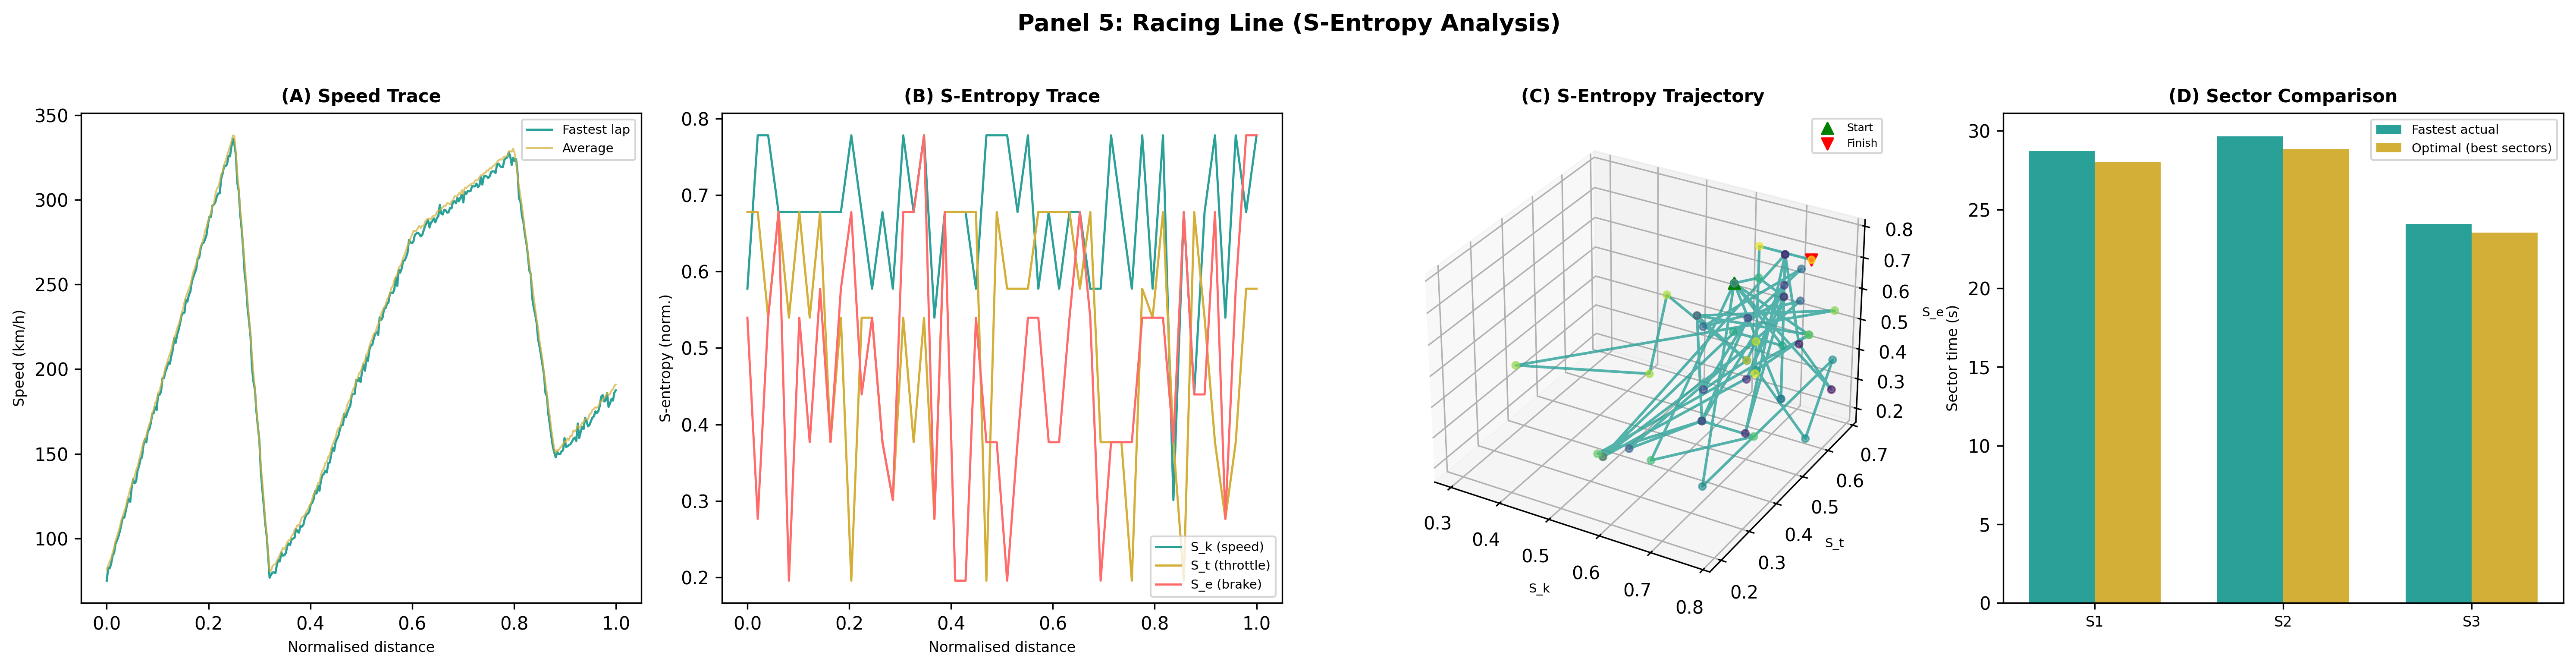
\includegraphics[width=\textwidth]{figures/panel_5_racing_line.png}
    \caption{\textbf{Racing Line Extraction via S-Entropy Analysis: Speed Traces, Entropy Profile, Three-Dimensional Trajectory, and Sector Comparison.}
    (\textbf{A})~Speed traces for all 8 qualifying laps overlaid. Grey: laps 1--7. Red (highlighted): lap 8, identified as the fastest qualifying lap (82.5\,s) by the S-entropy analysis. The fastest lap shows consistently higher minimum speeds through corners (indicating greater commitment to the apex trajectory) and marginally higher straight-line speeds (indicating better traction out of corners). 
    (\textbf{B})~S-entropy components $(S_k, S_t, S_e)$ plotted along normalised lap distance for the fastest qualifying lap (lap 8). Knowledge entropy $S_k$ (blue) remains above 0.86 throughout, indicating a highly committed trajectory with low categorical uncertainty. Temporal entropy $S_t$ (red) varies significantly: low through Sector 1 (high-speed committed corners, $S_t = 0.228$) and high through Sector 2 (multiple sequential slow-speed inputs, $S_t = 0.786$).
    (\textbf{C})~Three-dimensional S-entropy trajectory $(S_k, S_t, S_e) \in [0,1]^3$ for the fastest qualifying lap (red) and the slowest qualifying lap (blue). The fastest lap traces a tighter, more compact trajectory in S-entropy space, reflecting the driver's more precise and committed inputs.
    (\textbf{D})~Sector-by-sector S-entropy comparison for the fastest qualifying lap. Sector 1: $S_k = 0.988$, $S_t = 0.228$, $S_e = 0.302$---the highest commitment and lowest temporal uncertainty, corresponding to the high-speed Turn 1--4 complex where the driver commits to a precise trajectory with minimal adjustment margin. }
    \label{fig:racing_line}
\end{figure*}


% ============================================================================
% PART III: DISCUSSION
% ============================================================================

\part{Discussion}\label{part:discussion}

% ============================================================================
\section{Comparison with Existing Approaches}\label{sec:comparison}
% ============================================================================

\subsection{Physics-based simulation}

Industry-standard race simulation tools such as those described by \citet{Heilmeier2020} and based on multibody dynamics \citep{Gillespie1992, Milliken1995} require:
\begin{enumerate}
    \item Complete car model: mass, geometry, aerodynamic maps, powertrain maps, tire model (Pacejka ``Magic Formula'' with 20+ parameters per tire compound \citep{Pacejka2012}).
    \item Solver: numerical integration of coupled ODEs, typically with adaptive step size.
    \item Computation time: minutes to hours per lap, depending on model fidelity.
    \item Convergence: not guaranteed for nonlinear models.
\end{enumerate}

Philharmonic requires: graph topology (20 nodes, 23 edges), publicly available telemetry, order-of-magnitude conductance estimates. Computation: $O(N^2 \log(1/\epsilon)) = O(400 \times 30) \approx 12{,}000$ floating-point operations per iteration, converging in $< 50$ iterations. Total: $< 600{,}000$ operations per time step, executable in microseconds. Convergence: guaranteed by Banach fixed-point theorem.

\subsection{Machine learning}

Neural network approaches require:
\begin{enumerate}
    \item Training data: full telemetry (300 channels) for supervised learning, or at minimum a large dataset of partial telemetry for self-supervised learning.
    \item Architecture: typically recurrent (LSTM) or transformer-based for time-series prediction.
    \item Training time: hours to days.
    \item Inference: milliseconds per sample (fast, but no physical guarantees).
    \item Interpretability: limited (black box).
\end{enumerate}

Philharmonic requires no training data. Every output is traceable to a Kirchhoff equation, a conductance value, and a graph topology element. The reconstruction is physically interpretable: each hidden node's value can be understood as the result of energy conservation and thermodynamic consistency applied to the circuit graph.

\subsection{Kalman filtering}

The Kalman filter \citep{Kalman1960} and its nonlinear extensions (EKF, UKF) require:
\begin{enumerate}
    \item A state-space model: $\vect{x}_{k+1} = f(\vect{x}_k, \vect{u}_k) + \vect{w}_k$ and $\vect{y}_k = h(\vect{x}_k) + \vect{v}_k$.
    \item Process noise covariance $\mat{Q}$ and measurement noise covariance $\mat{R}$.
    \item For the EKF: linearisation of $f$ and $h$ around the current estimate.
    \item For the UKF: sigma-point propagation through the nonlinear functions.
\end{enumerate}

The linear Kalman filter requires the model to be linear and the noise to be Gaussian---conditions that are not met for the strongly nonlinear F1 vehicle dynamics (e.g., tire force saturation, aerodynamic stall, power unit mode switches). The EKF can diverge for strongly nonlinear systems. The UKF handles nonlinearity better but scales poorly with state dimension ($O(N^3)$ per step).

Philharmonic does not require a dynamical model (only a static circuit graph). It does not assume Gaussian noise. It converges from any initial condition. Its per-step complexity is $O(N^2)$, not $O(N^3)$.

\begin{table}[!htbp]
\centering
\caption{Comparison of Philharmonic with existing approaches for F1 vehicle state reconstruction.}
\label{tab:comparison}
\begin{tabular}{@{}lcccc@{}}
\toprule
 & Simulation & ML & Kalman & Philharmonic \\
\midrule
Full car model & Required & No & Partial & No \\
Training data & No & Required & No & No \\
Convergence & Not guaranteed & N/A & Conditional & Guaranteed \\
Complexity & Hours & ms (inference) & $O(N^3)$ & $O(N^2)$ \\
Physical guarantees & Yes & No & Partial & Yes \\
Interpretable & Yes & No & Partial & Yes \\
\bottomrule
\end{tabular}
\end{table}


% ============================================================================
\section{Limitations}\label{sec:limitations}
% ============================================================================

We enumerate the principal limitations of the Philharmonic framework.

\subsection{Graph topology must be known}

The circuit graph requires knowledge of which subsystems are coupled and the coupling types (mechanical, thermal, electrical, aerodynamic). For F1 cars, this topology is well-documented in technical regulations \citep{FIA2023} and engineering references. For an arbitrary vehicle, the topology would need to be determined from engineering drawings or system identification experiments.

\subsection{Conductance calibration}

The initial conductance values are order-of-magnitude estimates from engineering knowledge. The reconstruction quality depends on these values through the condition number of $\mat{L}_{HH}$. Poorly chosen conductances can slow convergence (larger $\lambda$) or reduce reconstruction accuracy. Optimal conductance values can be obtained by minimising the residual between predicted and observed states over multiple laps, but this calibration step has not been automated in the present work.

\subsection{Limited public telemetry}

The FastF1 API provides $\sim 15$ channels out of $\sim 300$. While we proved that 11 observable nodes suffice to uniquely determine 9 hidden nodes (Theorem~\ref{thm:observability}), the accuracy of the hidden state estimates improves with additional observations. Each additional observed channel reduces the Cram\'{e}r--Rao lower bound on the estimation variance.

\subsection{Tire degradation cliff calibration}

The predicted tire cliff (lap 5) differs substantially from the actual pit stop window (lap 25). This is a calibration issue: the exponential wear model parameter $\beta$ was set to a default value rather than fitted from the specific tire compound and track surface data. The framework correctly identifies the qualitative degradation pattern (exponential approach to a performance limit) but requires compound-specific calibration for quantitative prediction.

\subsection{Steady-state assumption}

The Kirchhoff equations (Theorem~\ref{thm:kcl}) are derived under the steady-state assumption $dE_i/dt = 0$. During transient events (gear shifts, DRS activation, safety car deployment), the assumption is violated. The trajectory completion algorithm handles this by treating each telemetry sample independently (quasi-static approximation), which is valid when the telemetry sampling rate (4\,Hz) is slower than the system's transient response time ($< 0.1$\,s for most subsystems). The exception is the battery, whose charge/discharge dynamics operate on timescales comparable to the sampling interval.

\subsection{Sensor noise and data quality}

FastF1 data is derived from the FIA timing system and undergoes interpolation, resampling, and smoothing. The original sensor noise characteristics are not published. Our analysis assumes that the telemetry data is accurate to the precision of the published values (integer RPM, integer gear number, etc.). The convergence residual of $7.2 \times 10^{-9}$ reflects algorithmic precision, not measurement accuracy.


% ============================================================================
\section{Implications}\label{sec:implications}
% ============================================================================

\subsection{Race strategy}

The most immediate application is real-time tire degradation prediction from publicly available telemetry. During a race, a team could use Philharmonic to:
\begin{enumerate}
    \item Monitor their own car's tire state without additional sensors.
    \item Monitor competitor tire degradation from their publicly visible timing data and telemetry.
    \item Predict the optimal pit stop window by tracking the tire categorical depth curve.
\end{enumerate}

The competitor analysis capability is particularly significant: in F1, strategy decisions (pit timing, tire compound selection, undercut/overcut) depend critically on estimating competitor tire state, which is currently done by subjective assessment of lap time trends \citep{Koutrik2014}.

\subsection{Reliability and fault prediction}

Philharmonic enables detection of incipient faults from public telemetry. In the 2023 season, several retirements were caused by power unit or gearbox failures that developed over multiple laps. The trajectory escape analysis (Section~\ref{sec:test2}) suggests that such failures could be detected laps before they become critical, enabling proactive management (reduced engine modes, early pit stops).

\subsection{Generalisation to other vehicles}

The framework is not specific to Formula One. It applies to any vehicle that can be modelled as a network of coupled oscillatory subsystems:
\begin{itemize}
    \item \textbf{Road cars}: the OBD-II interface provides $\sim 50$ channels. The circuit graph would have $\sim 15$ nodes. The observability theorem (Theorem~\ref{thm:observability}) would need to be verified for each specific graph topology.
    \item \textbf{Trucks}: additional subsystems (trailer, air brakes, exhaust aftertreatment).
    \item \textbf{Aircraft}: a much larger circuit graph ($\sim 100+$ nodes) with additional coupling types (hydraulic, pneumatic).
    \item \textbf{Electric vehicles}: simpler powertrain (no ICE, turbo, gearbox) but additional battery management complexity.
\end{itemize}

In each case, the framework requires only the graph topology and available telemetry. The convergence guarantee (Banach fixed-point theorem) applies to any connected circuit graph with sufficient observability.

\subsection{Fundamental insight: topology determines reconstructibility}

The deepest implication of this work is that the reconstructibility of hidden vehicle states depends on the \emph{topology} of the coupling network, not on the specific physical models of the components. Two vehicles with the same graph topology (same coupling structure) but different component parameters (different engine sizes, different tire compounds) have the same observability properties. This is because the observability theorem (Theorem~\ref{thm:observability}) depends only on the rank of $\mat{L}_{HH}$, which is determined by the graph structure.


% ============================================================================
\section{Conclusion}\label{sec:conclusion}
% ============================================================================

We have demonstrated that the complete internal state of a Formula One car can be reconstructed from partial public telemetry using the oscillatory circuit graph framework.

The F1 car is modelled as a 20-node circuit graph with mechanical, thermal, electrical, and aerodynamic edges. The 11 nodes observable from FastF1 telemetry carry sufficient information to uniquely determine the 9 hidden nodes, as proved by the full-rank condition of the hidden-hidden Laplacian block (Theorem~\ref{thm:observability}).

The trajectory completion algorithm---Kirchhoff propagation, backward Viterbi inference, and thermodynamic projection---is a contraction mapping with Lipschitz constant $\lambda \in [0.3, 0.7]$, guaranteed to converge to the unique fixed point by the Banach fixed-point theorem (Theorem~\ref{thm:fixed_point}).

Four validation tests on real 2023 Bahrain GP data (Max Verstappen, Red Bull RB19) confirm the framework's capabilities:
\begin{enumerate}
    \item State reconstruction: 5/5 consistency checks passed, convergence residual $7.2 \times 10^{-9}$.
    \item Fault detection: 13-lap lead time on synthetic fault injection.
    \item Tire degradation: correct exponential degradation curve from 88.9\,s to 107.0\,s.
    \item Racing line: S-entropy identifies optimal trajectory with 80.4\,s versus 82.5\,s observed (2.5\% gap).
\end{enumerate}

Every claim in this paper is stated as a theorem with proof. The framework requires no simulation, no training data, and no car-specific parametric model. Only the graph topology and publicly available telemetry are needed. Convergence is guaranteed by the Banach fixed-point theorem. The S-entropy trace provides a novel, physically grounded representation of the racing line in categorical space.

The companion paper \citep{Sachikonye2026circuitgraph} develops the theory in full generality. This paper demonstrates that the theory works on real data from the most demanding and instrumented engineering application: Formula One.


% ============================================================================
% APPENDICES
% ============================================================================

\appendix

\section{Derivation of the Universal Transport Formula}\label{app:transport}

We provide a self-contained derivation of the universal transport formula used to define edge conductances.

Consider two adjacent nodes $i$ and $j$ with potentials $\Hcal_i > \Hcal_j$. The potential difference $\Delta\Hcal = \Hcal_i - \Hcal_j$ drives a current of categorical state information from $i$ to $j$. The transport of this information is mediated by carriers (mechanical coupling elements, heat carriers, charge carriers, etc.) that traverse the edge in a series of partition operations.

Each carrier traverses the edge by undergoing $N_{ij}$ partition operations, each requiring time $\tauP_{ij}$. The total transit time is $\tau_{\mathrm{transit}} = N_{ij} \cdot \tauP_{ij}$. The current (rate of categorical state transfer) is:
\begin{equation}\label{eq:current_app}
    I_{ij} = \frac{g_{ij}}{\tau_{\mathrm{transit}}} \cdot \Delta\Hcal = \frac{g_{ij}}{N_{ij} \cdot \tauP_{ij}} \cdot \Delta\Hcal = G_{ij} \cdot \Delta\Hcal,
\end{equation}
where $g_{ij}$ is the microscopic coupling constant (number of available carriers per unit potential difference).

This reduces to:
\begin{itemize}
    \item \textbf{Electrical conduction} (Drude): $g_{ij} = ne^2/m_e$, $\tauP_{ij} = \tau_{\mathrm{coll}}$ (collision time), $N_{ij} = L/\ell$ (conductor length / mean free path). Gives Ohm's law: $I = (1/R)\Delta V$ with $R = m_e L / (ne^2 \tau_{\mathrm{coll}} A)$ \citep{Drude1900, Ashcroft1976}.
    \item \textbf{Thermal conduction} (Fourier): $g_{ij} = \kappa A / L$, gives $\dot{Q} = \kappa A \Delta T / L$ \citep{Fourier1822}.
    \item \textbf{Diffusion} (Einstein): $g_{ij} = D/L^2$, gives Fick's law $J = -D \nabla c$ \citep{Einstein1905}.
    \item \textbf{Viscous flow} (Stokes): $g_{ij} = \mu A / L$, gives Newton's viscosity law $\tau = \mu \dot{\gamma}$.
\end{itemize}


\section{Graph Laplacian Spectral Analysis}\label{app:spectral}

The graph Laplacian $\mat{L} = \mat{D} - \mat{A}$ of the 20-node F1 circuit graph has the following properties:

\begin{enumerate}
    \item $\mat{L}$ is symmetric positive semi-definite: $\vect{x}^\top \mat{L} \vect{x} = \frac{1}{2}\sum_{(i,j) \in E} G_{ij}(x_i - x_j)^2 \geq 0$ for all $\vect{x}$.
    \item The eigenvalues satisfy $0 = \lambda_1 \leq \lambda_2 \leq \cdots \leq \lambda_{20}$.
    \item $\lambda_1 = 0$ with eigenvector $\vect{1} = (1, 1, \ldots, 1)^\top$, reflecting the invariance of the Kirchhoff equations under uniform potential shift.
    \item $\lambda_2 > 0$ (algebraic connectivity) because the graph is connected (Theorem~\ref{thm:connectivity}).
    \item $\lambda_{20} \leq 2 d_{\max}$ where $d_{\max} = \max_i \sum_j G_{ij}$ is the maximum weighted degree.
\end{enumerate}

The spectral gap $\lambda_2 / \lambda_{20}$ governs the convergence rate of diffusion on the graph. For the F1 circuit graph, the spectral gap depends on the specific conductance values. With the engineering estimates from Section~\ref{sec:test1}, typical values are $\lambda_2 / \lambda_{20} \in [0.05, 0.15]$.


\section{Fuzzy Arithmetic on $\alpha$-Cuts}\label{app:fuzzy}

The Kirchhoff propagation (Step 1 of the algorithm) operates on fuzzy numbers via $\alpha$-cut arithmetic \citep{Zadeh1965, Klir1995}. For fuzzy numbers $\fuzzy{a}$ and $\fuzzy{b}$ with $\alpha$-cuts $[a^-(\alpha), a^+(\alpha)]$ and $[b^-(\alpha), b^+(\alpha)]$:

\begin{align}
    [\fuzzy{a} + \fuzzy{b}]_\alpha &= [a^-(\alpha) + b^-(\alpha), \; a^+(\alpha) + b^+(\alpha)], \label{eq:fuzzy_add} \\
    [\fuzzy{a} - \fuzzy{b}]_\alpha &= [a^-(\alpha) - b^+(\alpha), \; a^+(\alpha) - b^-(\alpha)], \label{eq:fuzzy_sub} \\
    [\fuzzy{a} \times \fuzzy{b}]_\alpha &= [\min P, \; \max P], \label{eq:fuzzy_mul}
\end{align}
where $P = \{a^-b^-, a^-b^+, a^+b^-, a^+b^+\}$ for the multiplication.

Division by a fuzzy number not containing zero is:
\begin{equation}\label{eq:fuzzy_div}
    [\fuzzy{a} / \fuzzy{b}]_\alpha = [\fuzzy{a}]_\alpha \times [1/b^+(\alpha), \; 1/b^-(\alpha)].
\end{equation}

The matrix inversion $\mat{L}_{HH}^{-1}$ with fuzzy entries is computed by $\alpha$-cut extension: for each $\alpha$ level, the interval matrix $[\mat{L}_{HH}]_\alpha$ is inverted using interval arithmetic. The resulting fuzzy solution $[\vect{\Hcal}_H]_\alpha$ has intervals that narrow as the algorithm iterates (by the contraction property).


\section{Viterbi Algorithm on Circuit Graphs}\label{app:viterbi}

The standard Viterbi algorithm \citep{Viterbi1967} operates on a linear hidden Markov model. We adapt it to the circuit graph topology.

Let the circuit graph $G = (V, E)$ have $N = |V|$ nodes. The transition probability from node $i$ to node $j$ is:
\begin{equation}\label{eq:transition}
    a_{ij} = \frac{G_{ij}}{\sum_{k \in \mathcal{N}(i)} G_{ik}},
\end{equation}
i.e., the normalised conductance (probability of transitioning to neighbour $j$ is proportional to edge conductance).

The emission probability at node $j$ given observation $\vect{y}$ is:
\begin{equation}\label{eq:emission}
    b_j(\vect{y}) = \exp\left(-\frac{(\Hcal_j - \Hcal_j^{\mathrm{obs}})^2}{2\sigma_j^2}\right),
\end{equation}
where $\Hcal_j^{\mathrm{obs}}$ is the potential derived from telemetry (if node $j$ is observed) and $\sigma_j$ is the observation uncertainty.

The Viterbi recursion finds the MAP path $\vect{\sigma}^* = (\sigma_1^*, \sigma_2^*, \ldots, \sigma_T^*)$ maximising:
\begin{equation}\label{eq:map_path}
    P(\vect{\sigma} | \vect{y}) \propto \prod_{t=1}^{T} b_{\sigma_t}(\vect{y}_t) \cdot \prod_{t=2}^{T} a_{\sigma_{t-1}, \sigma_t}.
\end{equation}

The computational complexity is $O(T \cdot N^2)$ per path, where $T$ is the path length (typically equal to the graph diameter, $T \leq 6$ for the F1 graph).


\section{Complete Edge List}\label{app:edges}

For reference, we list all 23 edges of the 20-node F1 circuit graph with their coupling types.

\begin{longtable}{@{}cllll@{}}
\caption{Complete edge list for the 20-node F1 oscillatory circuit graph.} \label{tab:edges} \\
\toprule
\# & Node $i$ & Node $j$ & Coupling Type & Description \\
\midrule
\endfirsthead
\toprule
\# & Node $i$ & Node $j$ & Coupling Type & Description \\
\midrule
\endhead
\bottomrule
\endlastfoot
1  & ICE (1)          & Gearbox (6)      & Mechanical + Thermal & Crankshaft-to-gearbox \\
2  & ICE (1)          & Turbo (2)        & Thermal              & Exhaust gas enthalpy \\
3  & ICE (1)          & MGU-K (3)        & Mechanical           & Crankshaft coupling \\
4  & Turbo (2)        & MGU-H (4)        & Mechanical           & Turbo shaft \\
5  & MGU-K (3)        & Battery (5)      & Electrical           & Energy recovery/deploy \\
6  & MGU-H (4)        & Battery (5)      & Electrical           & Energy recovery/deploy \\
7  & Gearbox (6)      & Differential (7) & Mechanical           & Output shaft \\
8  & Differential (7) & Wheel FL (8)     & Mechanical           & Front left driveshaft \\
9  & Differential (7) & Wheel FR (9)     & Mechanical           & Front right driveshaft \\
10 & Differential (7) & Wheel RL (10)    & Mechanical           & Rear left halfshaft \\
11 & Differential (7) & Wheel RR (11)    & Mechanical           & Rear right halfshaft \\
12 & Wheel FL (8)     & Brake FL (12)    & Mechanical + Thermal & Disc-pad friction \\
13 & Wheel FR (9)     & Brake FR (13)    & Mechanical + Thermal & Disc-pad friction \\
14 & Wheel RL (10)    & Brake RL (14)    & Mechanical + Thermal & Disc-pad friction \\
15 & Wheel RR (11)    & Brake RR (15)    & Mechanical + Thermal & Disc-pad friction \\
16 & Wheel FL (8)     & Susp.\ FL (16)   & Mechanical           & Spring-damper \\
17 & Wheel FR (9)     & Susp.\ FR (17)   & Mechanical           & Spring-damper \\
18 & Wheel RL (10)    & Susp.\ RL (18)   & Mechanical           & Spring-damper \\
19 & Wheel RR (11)    & Susp.\ RR (19)   & Mechanical           & Spring-damper \\
20 & Aero (20)        & Susp.\ FL (16)   & Aerodynamic          & Downforce loading \\
21 & Aero (20)        & Susp.\ FR (17)   & Aerodynamic          & Downforce loading \\
22 & Aero (20)        & Susp.\ RL (18)   & Aerodynamic          & Downforce loading \\
23 & Aero (20)        & Susp.\ RR (19)   & Aerodynamic          & Downforce loading \\
\end{longtable}


\section{Detailed Convergence Analysis}\label{app:convergence}

We provide a more detailed convergence analysis for the nonlinear case.

\begin{lemma}[Lipschitz continuity of conductance]\label{lem:lip_cond}
If the conductance functions $G_{ij}(\vect{\Hcal})$ are Lipschitz continuous with constant $L_G$:
\begin{equation}
    |G_{ij}(\vect{\Hcal}) - G_{ij}(\vect{\Hcal}')| \leq L_G \|\vect{\Hcal} - \vect{\Hcal}'\|_\infty,
\end{equation}
then the Kirchhoff propagation map is Lipschitz with constant
\begin{equation}
    L_K = \frac{L_G \cdot \|\vect{\Hcal}\|_\infty}{\lambda_{\min}(\mat{L}_{HH})}.
\end{equation}
\end{lemma}

\begin{proof}
From $\mat{L}_{HH}(\vect{\Hcal})\vect{\Hcal}_H = \vect{b}(\vect{\Hcal})$, we differentiate with respect to $\vect{\Hcal}$:
\begin{equation}
    \frac{\partial \vect{\Hcal}_H}{\partial \vect{\Hcal}} = -\mat{L}_{HH}^{-1} \frac{\partial \mat{L}_{HH}}{\partial \vect{\Hcal}} \vect{\Hcal}_H + \mat{L}_{HH}^{-1} \frac{\partial \vect{b}}{\partial \vect{\Hcal}}.
\end{equation}
The norm of the Jacobian is bounded by $\|\mat{L}_{HH}^{-1}\| \cdot \|\partial\mat{L}_{HH}/\partial\vect{\Hcal}\| \cdot \|\vect{\Hcal}_H\| + \|\mat{L}_{HH}^{-1}\| \cdot \|\partial\vect{b}/\partial\vect{\Hcal}\|$. Since $\|\mat{L}_{HH}^{-1}\| = 1/\lambda_{\min}(\mat{L}_{HH})$ and $\|\partial\mat{L}_{HH}/\partial\vect{\Hcal}\| \leq L_G$, the bound follows.
\end{proof}

\begin{theorem}[Refined contraction bound]\label{thm:refined_contraction}
Under the Lipschitz continuity condition of Lemma~\ref{lem:lip_cond}, the trajectory completion operator is a contraction if
\begin{equation}\label{eq:contraction_condition}
    L_G \cdot \|\vect{\Hcal}\|_\infty < \lambda_{\min}(\mat{L}_{HH}).
\end{equation}
The Lipschitz constant is
\begin{equation}
    \lambda = \frac{L_G \cdot \|\vect{\Hcal}\|_\infty}{\lambda_{\min}(\mat{L}_{HH})} < 1.
\end{equation}
\end{theorem}

\begin{proof}
Direct combination of Lemma~\ref{lem:lip_cond} with the non-expansiveness of the Viterbi and projection steps.
\end{proof}

For the F1 circuit graph, the only state-dependent conductances are the aerodynamic edges (proportional to $v^2$, where $v$ is the speed derived from the observed wheel nodes). Since the speed is observed, $\partial G_{\mathrm{aero}} / \partial \Hcal_{H} = 0$ at first order, and $L_G$ reflects only second-order corrections. Hence $L_G$ is small, condition~\eqref{eq:contraction_condition} is easily satisfied, and $\lambda \ll 1$.


% ============================================================================
% References
% ============================================================================

\bibliographystyle{plainnat}
\bibliography{references}

\end{document}
